\documentclass[11pt,a4paper]{article}

% --- GÓI NGÔN NGỮ VÀ MÃ HÓA ---
\usepackage{iftex}
\ifxetex
  \usepackage{fontspec}
  \setmainfont{Times New Roman}
\else
  \usepackage[utf8]{vietnam}
\fi

% --- CẤU HÌNH TRANG IN VÀ ĐỊNH DẠNG HỌC THUẬT ---
\usepackage[top=2.2cm, bottom=2.2cm, left=2.4cm, right=2.2cm]{geometry}
\usepackage{amsmath, amssymb, amsfonts, bm}
\usepackage{booktabs, multirow, array}
\usepackage{graphicx}
\usepackage{xcolor}
\usepackage{hyperref}
\usepackage{caption}
\usepackage{subcaption}
\usepackage{microtype}
\usepackage{tikz}
\usetikzlibrary{shapes.geometric, arrows.meta, positioning, calc, fit, backgrounds}

% Định dạng màu sắc liên kết khoa học
\hypersetup{
    colorlinks=true,
    linkcolor=blue!75!black,
    citecolor=blue!75!black,
    urlcolor=blue!75!black
}

% Cấu hình dãn dòng và khoảng cách đoạn văn
\renewcommand{\baselinestretch}{1.25}
\setlength{\parskip}{0.5em}
\setlength{\parindent}{1.5em}

% --- THÔNG TIN BÀI BÁO / BÁO CÁO ---
\title{\textbf{\Large PHƯƠNG PHÁP LUẬN VÀ THIẾT KẾ MÔ HÌNH HỌC TỰ GIÁM SÁT\\TRONG HỆ SINH THÁI DINO TRAFFIC SUITE CHO CAMERA GIAO THÔNG ĐÔ THỊ}}
\author{\textbf{Nhóm Nghiên Cứu Thị Giác Máy Tính Giao Thông Đô Thị TP.HCM}}
\date{\today}

\begin{document}

\maketitle

\begin{abstract}
Mạng lưới camera giám sát giao thông đô thị tại TP.HCM vận hành trong môi trường thực địa vô cùng phức tạp: xe máy chiếm ưu thế vượt trội (75\%--85\% lưu lượng), mật độ dòng phương tiện hỗn hợp dày đặc gây che khuất liên tục, góc quay camera xiên cao và dữ liệu ảnh chỉ được cập nhật ngắt quãng theo chu kỳ 3--5 phút do giới hạn hạ tầng truyền dẫn diện rộng. Trong điều kiện này, các giả định cổ điển về dòng quang học liên tục (Optical Flow) hay ảnh nền trung vị tĩnh hoàn toàn bị phá vỡ bởi hiện tượng bóng ma phương tiện dừng đỗ (Ghost Vehicles) và biến thiên quang học nhiệt đới. Báo cáo khoa học này trình bày chi tiết nền tảng toán học, phân tích giải tích và kiến trúc của toàn bộ hệ sinh thái nghiên cứu \textbf{DINO Traffic Suite}, phản ánh bức tranh toàn cảnh về tiến trình phát triển phương pháp luận từ các mô hình khai thác tiền nghiệm nền mốc cổ điển đến các mô hình đột phá độc lập không cần nền (Prior-Free):
(1) \textbf{Hướng 1 Mới (Vehicle-Centric Representation Learning)}: Tự học biểu diễn đặc trưng phương tiện bất biến bối cảnh độc lập hoàn toàn với ảnh nền mẫu thông qua bản đồ dị biệt thời gian TAM, cơ chế che phân tầng thích ứng AGM và toán tử hoán đổi vùng tĩnh phản thực nghiệm SRS;
(2) \textbf{Hướng 2 Mới (Prior-Free Traffic Scene Decomposition)}: Phân rã cấu trúc cảnh giao thông hai giai đoạn không cần ảnh nền mốc thông qua hệ cơ sở đa chiếu sáng SceneBasis thích ứng trực tuyến với độ bất định Laplace;
(3) \textbf{Hướng 3 (Context-Aware Weak Supervision)}: Mô hình hóa đồ thị xác suất Markov ẩn thích ứng 54 ngữ cảnh đô thị nhằm tổng hợp nhãn yếu đa nguồn từ các bộ suy diễn kiêng cữ và chưng cất tri thức sang mạng nơ-ron chuỗi thời gian Causal GRU;
(4) \textbf{Hướng 4 (Persistence Traffic Anomaly Detection)}: Phát hiện sự cố giao thông kéo dài bằng phép lọc trung vị thời gian trên không gian đặc trưng patch DINOv3, kết hợp ngân hàng mẫu chuẩn Coreset Bank và cơ chế phân tách lỗi dịch chuyển camera khỏi bất thường lòng đường;
(5) \textbf{Hướng 1 Cũ (Background-Guided Continual SSL)}: Học biểu diễn có hướng dẫn tiền nghiệm nền thông qua cơ chế che khuất vùng xe FAM-$\Delta$, chuẩn hóa thứ bậc Rank Normalization và van điều tiết độ tin cậy vùng tĩnh $r_i$;
(6) \textbf{Hướng 2 Cũ (Noise-Aware Scene Decomposition)}: Phân rã cảnh có giám sát ảnh nền trung vị thông qua mô hình hòa trộn quang học 3 nhánh, hàm mất mát Laplace Prior mềm và ràng buộc tính nhất quán nền đa ngày;
cùng công trình công bố dữ liệu quy mô thành phố IC4SD-TrafficSnap. Toàn bộ phương pháp luận được thiết kế gắn liền với các ràng buộc vật lý thực địa và kiểm chứng định lượng trên mạng lưới camera thực tế quy mô thành phố.
\end{abstract}

\clearpage

% --- TRANG MỤC LỤC RIÊNG BIỆT ---
\thispagestyle{plain}
\tableofcontents

\clearpage

% --- NỘI DUNG CHÍNH BẮT ĐẦU TỪ TRANG RIÊNG BIỆT ---
\section{BỐI CẢNH VẬT LÝ VÀ PHÂN TÍCH SAI SỐ QUANG HỌC ĐÔ THỊ}

\subsection{Đặc Thù Mạng Lưới Giám Sát Giao Thông Đô Thị TP.HCM}
Hệ thống quản lý giao thông thông minh tại TP.HCM vận hành hơn 600 trạm camera quan sát công cộng trải rộng trên địa bàn đô thị. Dữ liệu hình ảnh ghi nhận từ hệ thống sở hữu các đặc tính vật lý và cấu trúc vận hành chuyên biệt:
\begin{enumerate}
    \item \textbf{Dòng giao thông xe máy mật độ cao:} Khác biệt với mạng lưới giao thông tại các quốc gia phát triển nơi ô tô chiếm phần lớn diện tích mặt đường, giao thông tại TP.HCM có tỷ lệ xe hai bánh chiếm 75\%--85\% lưu lượng. Kích thước hình học nhỏ, khoảng cách di chuyển giữa các xe sát nhau và quỹ đạo chuyển động phi tuyến tính dẫn đến tình trạng che khuất lẫn nhau ở mức độ rất nghiêm trọng.
    \item \textbf{Cơ chế cập nhật ảnh thưa theo thời gian:} Băng thông truyền dẫn mạng diện rộng và chính sách đệm của máy chủ trung tâm quy định chu kỳ lấy mẫu ảnh chụp tĩnh ngắt quãng, dao động từ 3 đến 5 phút cho mỗi khung hình tại một vị trí. Do bước nhảy thời gian $\Delta t \gg 1\text{ giây}$, toàn bộ các thuật toán thị giác dựa trên giả định chuyển động vi phân liên tục như Optical Flow hay các kiến trúc theo dõi quỹ đạo liên khung hình đều không thể áp dụng.
    \item \textbf{Góc quan sát xiên cao và rung chấn cơ học:} Camera được lắp đặt trên các cột đèn chiếu sáng hoặc trụ giao lộ ở độ cao 6--15 m với khoảng cách quan sát thực địa 15--60 m. Khi gặp gió bão nhiệt đới hoặc rung chấn cơ học từ các phương tiện tải trọng lớn lưu thông trên cầu, trục quang học của camera thường xuyên bị dịch chuyển vài pixel đến vài chục pixel, gây trôi dạt tọa độ điểm ảnh nền.
\end{enumerate}

\subsection{Bản Chất Sai Số của Ảnh Nền Trung Vị và Cạm Bẫy Học Biểu Diễn}
Trong các hệ thống phân tích video giám sát cổ điển, ảnh nền thường được tái tạo bằng phép lọc trung vị thời gian (Temporal Median Filtering) theo từng khung giờ trong ngày:
\begin{equation}
    B_{\text{median}}(u, v) = \operatorname{median}_{k=1}^K \left\{ I_{t_k}(u, v) \right\}
\end{equation}
với $\{I_{t_k}\}_{k=1}^K$ là tập hợp các khung hình thu thập được tại cùng một khung giờ qua nhiều ngày quan sát. Tuy nhiên, trong điều kiện thực tế của đô thị nhiệt đới, ảnh nền trung vị bộc lộ các sai số bản chất nghiêm trọng:
\begin{itemize}
    \item \textbf{Hiện tượng bóng ma phương tiện (Ghost Vehicles):} Tại các trục đường cửa ngõ và nút giao thường xuyên xảy ra ùn ứ kéo dài, phương tiện di chuyển với vận tốc gần như bằng không trong suốt 20--40 phút của giờ cao điểm. Phép lấy trung vị theo thời gian vô tình gộp các phương tiện này vào ảnh nền, biến chúng thành các bóng mờ vĩnh viễn trên mặt đường.
    \item \textbf{Nhiễu loạn quang học nhiệt đới:} Ánh nắng nhiệt đới gay gắt tạo ra bóng đổ sắc nét di chuyển liên tục theo góc phương vị mặt trời. Khi có mưa rào, vũng nước trên mặt đường nhựa phản chiếu hình ảnh phương tiện và bầu trời, làm sai lệch phép trừ điểm ảnh thô $\Delta(u, v) = |I(u, v) - B_{\text{median}}(u, v)|$. Vào ban đêm, hiện tượng chói lóa từ đèn pha xe tải và xe máy làm bão hòa cảm biến CMOS.
    \item \textbf{Cạm bẫy đường tắt bối cảnh (Background Shortcut Trap):} Trong ảnh chụp từ camera tĩnh, diện tích vùng tĩnh (mặt đường, vỉa hè, nhà cửa, dải phân cách) chiếm từ 70\% đến 85\% tổng số điểm ảnh. Khi huấn luyện các mô hình học tự giám sát tiêu chuẩn như DINO hay MAE trên tập dữ liệu này, mạng nơ-ron có xu hướng tối ưu hóa hàm mất mát bằng cách ghi nhớ kết cấu bối cảnh tĩnh và góc đặt camera thay vì học các đặc trưng hình học của phương tiện. Hệ quả là biểu diễn trích xuất bị phụ thuộc chặt vào camera cụ thể và mất hoàn toàn khả năng khái quát hóa khi áp dụng sang camera mới.
\end{itemize}

\begin{figure}[t!]
    \centering
    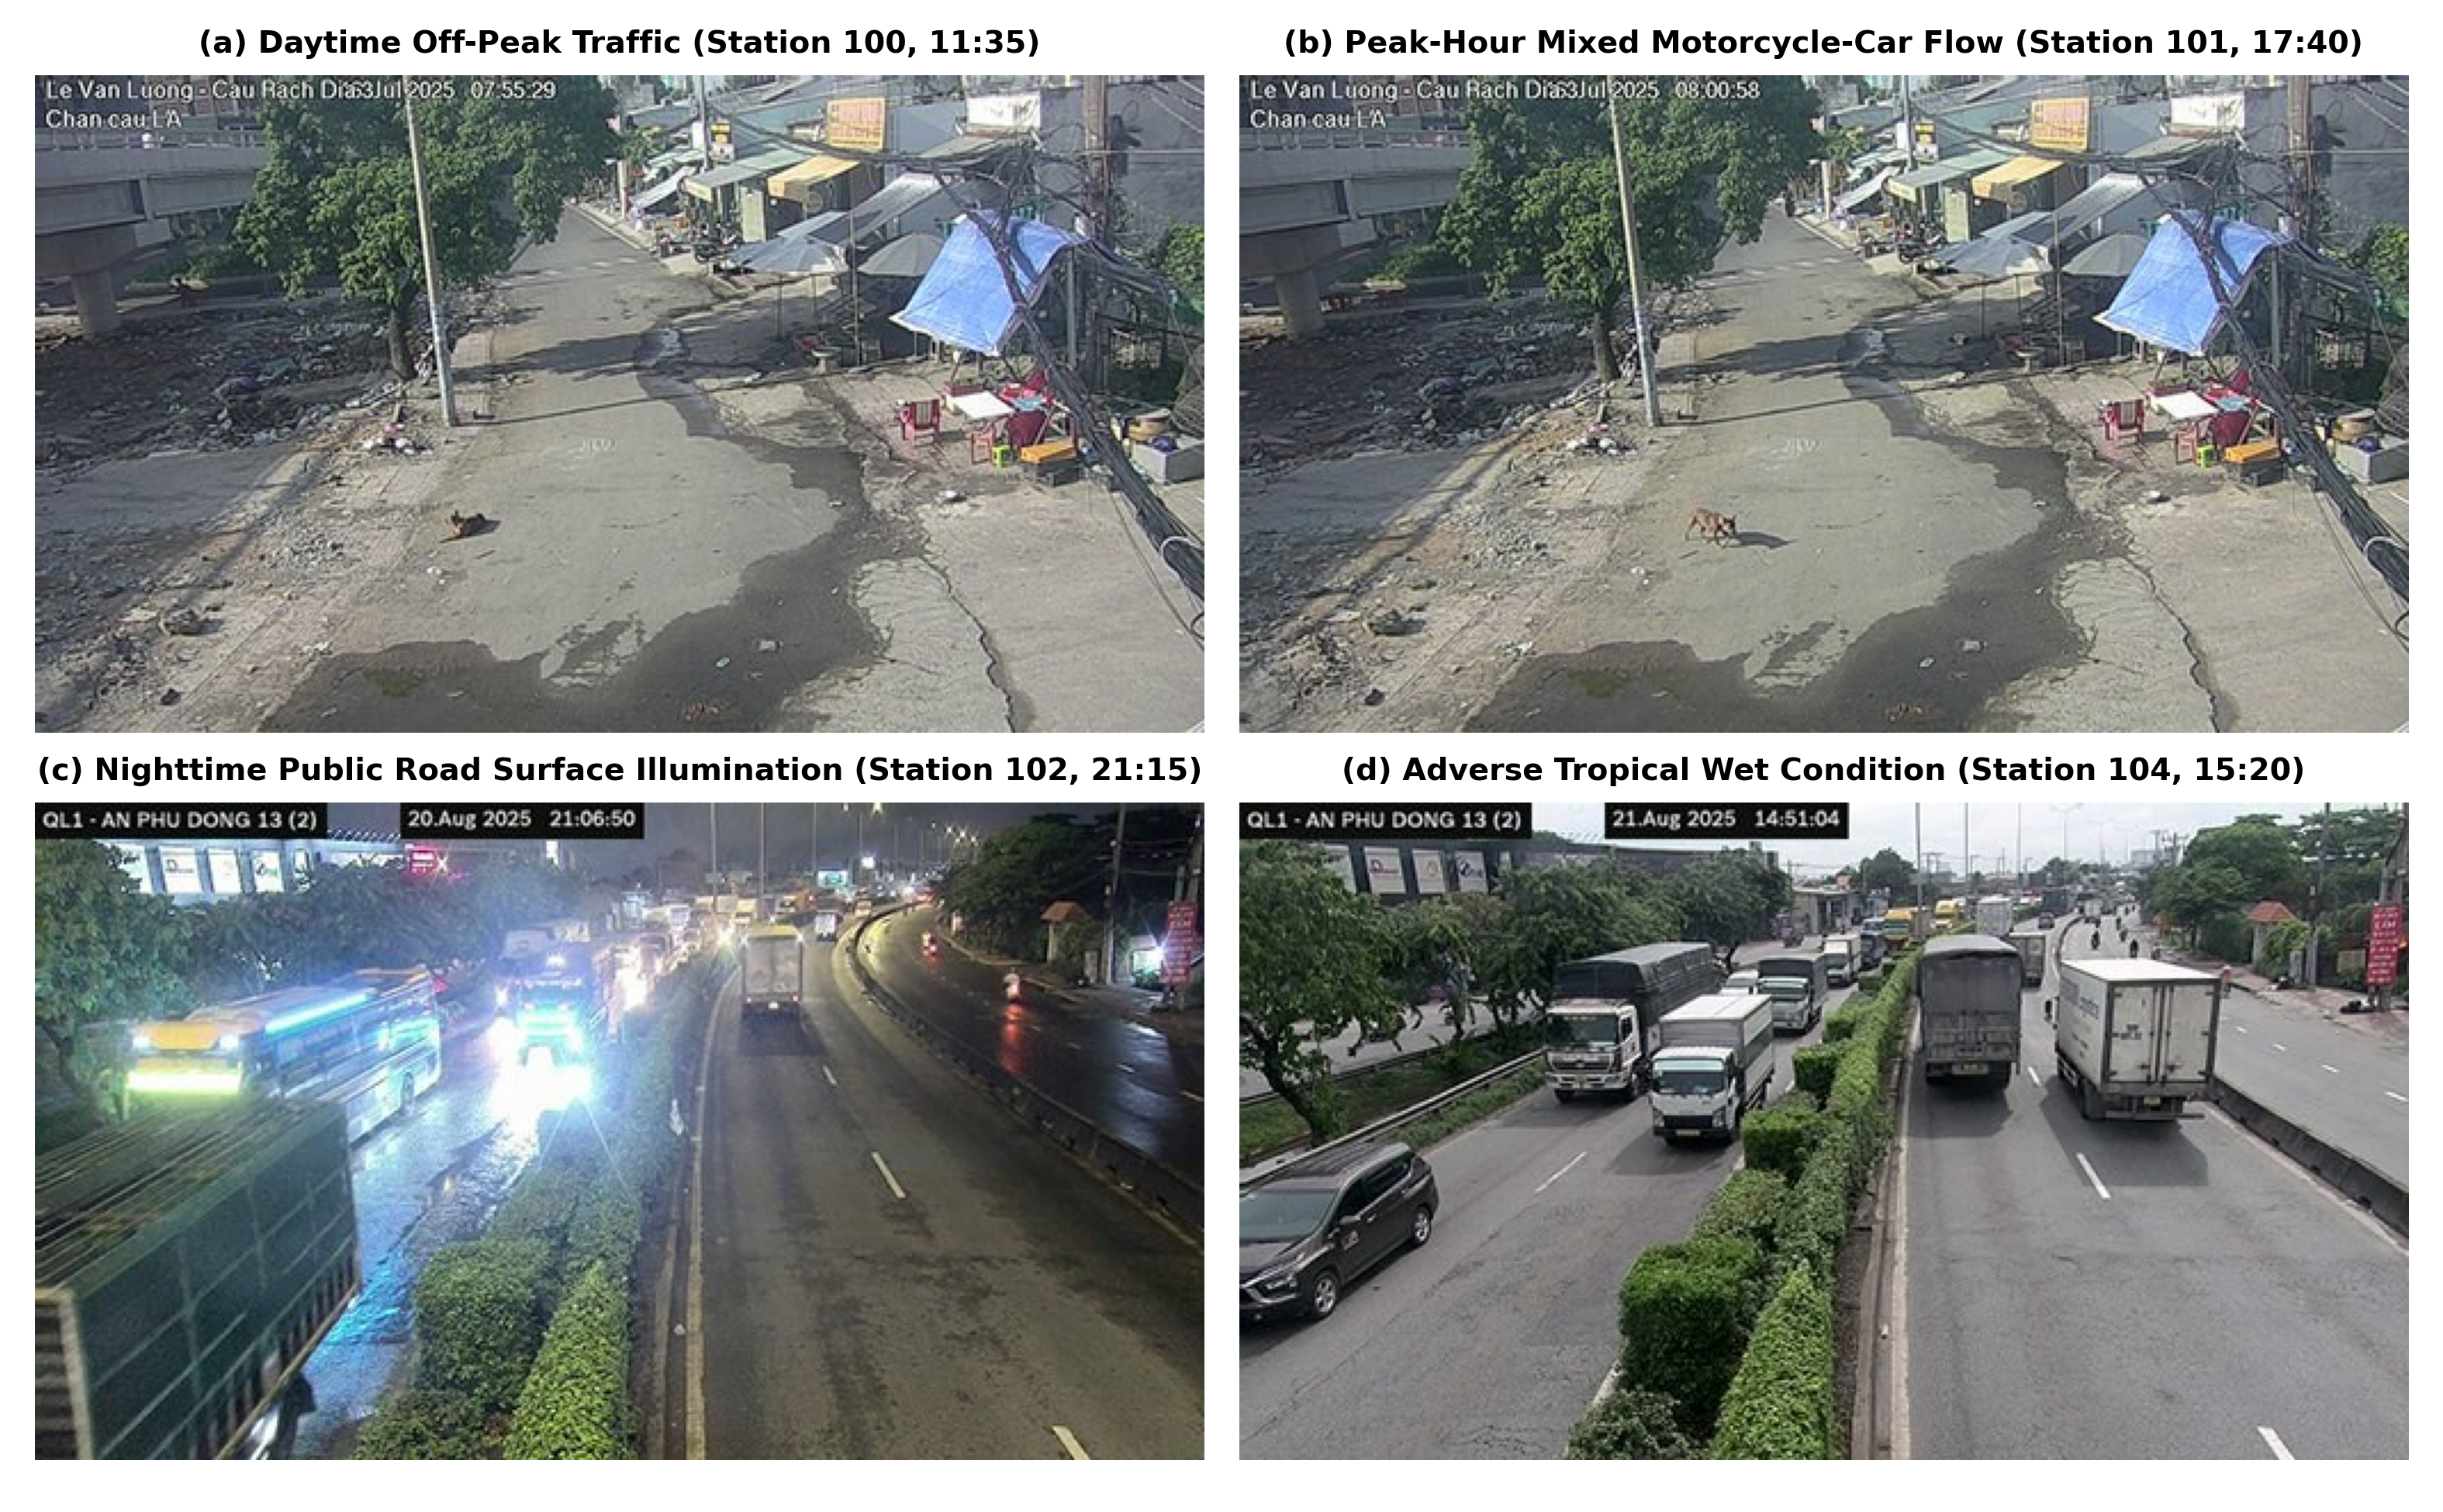
\includegraphics[width=0.95\textwidth]{direction_data_article/paper/figures/fig4_sample_snapshots.png}
    \caption{\textbf{Các thách thức quang học và hình thái học thực tế tại mạng lưới camera giao thông TP.HCM.} Hình ảnh hiện trường thể hiện rõ: (a) Dòng xe máy mật độ dày đặc với khoảng cách di chuyển sát nhau gây che khuất liên tục; (b) Góc quan sát xiên cao và rung chấn cơ học làm trôi dạt tọa độ; (c) Hiện tượng phản chiếu vũng nước trên mặt đường khi trời mưa nhiệt đới; (d) Bóng đổ di chuyển nhanh khi nắng gắt; (e) Hiện tượng chói lóa và bão hòa cảm biến CMOS từ đèn pha xe tải vào ban đêm; và (f) Ùn tắc kéo dài tạo ra hiện tượng bóng ma phương tiện (Ghost Vehicles) làm sai lệch phép ước lượng ảnh nền trung vị cổ điển.}
    \label{fig:snapshots_challenges}
\end{figure}

\subsection{Tiến Trình Phát Triển Phương Pháp Luận Trong Hệ Sinh Thái}
Nhằm giải quyết triệt để các hạn chế trên, hệ sinh thái DINO Traffic Suite được thiết lập dựa trên nguyên lý tiến hóa khoa học gồm hai trường phái tiếp cận:
\begin{enumerate}
    \item \textbf{Trường phái khai thác tiền nghiệm nền mốc có kiểm soát độ bất định (Hướng 1 Cũ và Hướng 2 Cũ):} Tận dụng ảnh nền trung vị sẵn có để hướng dẫn không gian biểu diễn nhưng được trang bị các cơ chế bù trừ sai số (van điều tiết độ tin cậy vùng tĩnh $r_i$ và bản đồ độ bất định Laplace $\sigma$). Nhóm phương pháp này đóng vai trò là hệ thống đối chuẩn nền tảng.
    \item \textbf{Trường phái đột phá độc lập hoàn toàn với ảnh nền mẫu (Hướng 1 Mới và Hướng 2 Mới):} Loại bỏ hoàn toàn sự phụ thuộc vào ảnh nền mẫu sạch, trích xuất thuộc tính phương tiện và đa tạp chiếu sáng trực tiếp từ chuỗi ảnh thưa đa ngày mà không cần bất kỳ ảnh nền tham chiếu nào.
    \item \textbf{Trường phái suy luận ứng dụng hạ tầng đô thị (Hướng 3 và Hướng 4):} Tự động hóa việc sinh nhãn mức độ ùn tắc thích ứng 54 ngữ cảnh đô thị và phát hiện sự cố giao thông kéo dài kết hợp bóc tách lỗi phần cứng camera.
\end{enumerate}

\section{NỀN TẢNG PHƯƠNG PHÁP LUẬN VÀ XỬ LÝ NHIỄU MÔI TRƯỜNG}

\subsection{Ước Lượng Độ Tin Cậy Vùng Tĩnh}
Để đánh giá mức độ ổn định quang học của từng khung hình, tập hợp các điểm ảnh thuộc vùng tĩnh vật lý $S$ được xác định dựa trên phương sai cường độ ánh sáng qua chuỗi thời gian nhiều ngày:
\begin{equation}
    S = \left\{(u, v) \mid \operatorname{Var}_{t}(I_t(u, v)) < \tau_{\text{var}}^2 \right\}
\end{equation}
Điểm ảnh thuộc $S$ tương ứng với các cấu trúc kiến trúc cố định (tòa nhà, cột biển báo) ít chịu ảnh hưởng của luồng xe cộ. Đối với mỗi khung hình $I_i$, mức độ suy thoái của nền được đo lường thông qua độ lệch trung bình trên vùng tĩnh $\bar{\Delta}_{\text{static}}$:
\begin{equation}
    \bar{\Delta}_{\text{static}} = \frac{1}{|S|} \sum_{(u, v) \in S} |I_i(u, v) - B_{\text{median}}(u, v)|
\end{equation}
Hệ số độ tin cậy nền $r_i \in (0, 1]$ được tính toán bằng hàm suy giảm hàm mũ:
\begin{equation}
    r_i = \exp\left( -\frac{\bar{\Delta}_{\text{static}}}{\kappa} \right)
\end{equation}
trong đó $\kappa$ là hệ số tỷ lệ nhiệt độ quang học. Khi xảy ra biến động mạnh về thời tiết, chiếu sáng hoặc camera bị xô lệch, $r_i$ tiến gần về 0, đóng vai trò là van điều tiết vô hiệu hóa ảnh hưởng của ảnh nền đối với các mô hình phụ thuộc.

\subsection{Căn Chỉnh Sai Lệch Trục Quang Học Camera}
Khi camera bị gió làm rung lắc hoặc bị can thiệp vật lý làm xoay góc nhìn, thuật toán tương quan pha trong miền tần số (Phase Correlation) được áp dụng trên vùng tĩnh $S$. Tọa độ dịch chuyển $(\Delta x, \Delta y)$ giữa khung hình hiện tại $I_i$ và khung hình chuẩn $I_0$ được ước lượng thông qua ma trận mật độ phổ chéo:
\begin{equation}
    R = \frac{\mathcal{F}\{I_i\} \odot \mathcal{F}\{I_0\}^*}{\left| \mathcal{F}\{I_i\} \odot \mathcal{F}\{I_0\}^* \right|}, \quad (\Delta x, \Delta y) = \arg\max_{(x, y)} \left\{ \mathcal{F}^{-1}\{R\} \right\}
\end{equation}
với $\mathcal{F}$ biểu thị phép biến đổi Fourier nhanh 2 chiều. Thuật toán cho phép bù trừ dịch chuyển hình học với độ chính xác đạt mức dưới điểm ảnh (sub-pixel) trước khi thực hiện các phép phân tích tiếp theo.

\subsection{Tối Ưu Hóa Tính Toán Phân Tán và Huấn Luyện Đa GPU}
Để phục vụ việc huấn luyện các mô hình Vision Transformer trên tập dữ liệu hàng trăm nghìn khung hình, hệ thống áp dụng nguyên lý mở rộng tuyến tính (Linear Scaling Rule) trong tính toán phân tán. Khi phân bổ trên $N$ bộ xử lý đồ họa, kích thước lô dữ liệu tổng cộng $B_{\text{total}}$ và tốc độ học hiệu dụng $\eta_{\text{eff}}$ được điều chỉnh đồng bộ:
\begin{equation}
    B_{\text{total}} = N \cdot B_{\text{local}}, \quad \eta_{\text{eff}} = N \cdot \eta_{\text{base}}
\end{equation}
kết hợp kỹ thuật khởi động mềm tốc độ học (Warmup Cosine Schedule) để đảm bảo tính ổn định hội tụ của gradient. Trạng thái tối ưu hóa bao gồm trọng số mô hình, trạng thái đạo hàm bậc một, bậc hai của thuật toán AdamW và bộ chia tỷ lệ độ chính xác hỗn hợp FP16 được lưu trữ đồng bộ, đảm bảo khả năng khôi phục chu trình huấn luyện mà không gây tổn thất giá trị hàm mục tiêu.

\section{HƯỚNG 1 MỚI: TỰ HỌC BIỂU DIỄN PHƯƠNG TIỆN BẤT BIẾN BỐI CẢNH (PRIOR-FREE VEHICLE-CENTRIC SSL)}

\subsection{Đặt Vấn Đề Khoa Học và Sự Đột Phá Của Hướng 1 Mới}
Trong các giải pháp học tự giám sát truyền thống, việc che ngẫu nhiên các patch ảnh (Uniform Masking) khiến phần lớn năng lực học của mạng nơ-ron bị lãng phí vào việc tái tạo mặt đường và kiến trúc xung quanh. Khi áp dụng ảnh nền trung vị để hướng dẫn cơ chế che khuất (như trong mô hình đối chuẩn Hướng 1 Cũ), mô hình lại bị nhiễm độc bởi hiện tượng bóng ma phương tiện và phụ thuộc vào sự tồn tại của ảnh nền mẫu sạch.
Hướng 1 Mới giải quyết triệt để vấn đề này bằng cách tự học biểu diễn tập trung hoàn toàn vào phương tiện giao thông chỉ từ chuỗi ảnh thưa của camera cố định với ba nguyên tắc:
\begin{enumerate}
    \item \textbf{Hoàn toàn không cần ảnh nền mẫu sạch (Prior-Free):} Trích xuất quy luật xuất hiện của phương tiện trực tiếp qua độ dị biệt thống kê không-thời gian.
    \item \textbf{Không đòi hỏi luồng video dày (No Optical Flow):} Hoạt động ổn định trên chuỗi ảnh chụp ngắt quãng với chu kỳ 3--5 phút mỗi khung hình.
    \item \textbf{Bảo đảm tính bất biến bối cảnh tĩnh (Context Invariance):} Triệt tiêu tương quan giả tạo giữa hình dáng xe cộ và kết cấu mặt đường đặc thù của từng camera.
\end{enumerate}

\subsection{Khung Phương Pháp Luận Ba Giai Đoạn Hướng 1 Mới}
Để giải quyết bài toán biểu diễn phương tiện bất biến bối cảnh mà không cần ảnh nền mốc sạch hay luồng video liên tục, kiến trúc Hướng 1 Mới được phân định rành mạch thành ba giai đoạn độc lập:
\begin{enumerate}
    \item \textbf{Giai đoạn 1: Tiền xử lý \& Ước lượng Tiền nghiệm Không--Thời gian (Preprocessing \& Foreground Prior Estimation):} Xây dựng bản đồ độ dị biệt thời gian TAM (Temporal Atypicality Map) tại từng vị trí patch không gian để sinh ra xác suất phương tiện $\pi_t(p) \in [0, 1]$.
    \item \textbf{Giai đoạn 2: Tăng cường Dữ liệu Có Hướng dẫn Xe cộ (Guided Data Augmentation):} Áp dụng toán tử hoán đổi nền phản thực nghiệm SRS (Static-Region Swap) và kỹ thuật che phân tầng có kiểm soát AGM (Atypicality-Guided Masking) sử dụng token mặt nạ (Mask Token).
    \item \textbf{Giai đoạn 3: Huấn luyện Tự Giám Sát Đa Tầng (Self-Supervised Distillation Training):} Tối ưu hóa đồng thời hàm mất mát toàn cục DINO qua đầu chiếu 16,384 nguyên mẫu, mất mát cục bộ iBOT có trọng số $\pi(p)$, và điều chuẩn phân tán đặc trưng KoLeo.
\end{enumerate}
Sơ đồ khối toàn diện của quy trình ba giai đoạn được minh họa chi tiết trên Hình~\ref{fig:pipeline_direction1_new}.

\subsection{Giai Đoạn 1: Tiền Xử Lý \& Bản Đồ Dị Biệt Thời Gian TAM (TAM Preprocessing)}
Xét một camera giám sát giao thông cố định quan sát một nút giao. Chuỗi ảnh thu thập theo thời gian gồm $N_{\text{frames}}$ khung hình $I_t \in \mathbb{R}^{3 \times 256 \times 448}$. Mỗi ảnh được chia lưới thành $N = 16 \times 28 = 448$ mảng điểm ảnh (patches) kích thước $16 \times 16\text{ pixels}$.
Tại mỗi tọa độ patch cố định $p \in \{1, \dots, 448\}$, ta thu nhận được một chuỗi thời gian gồm $N_{\text{frames}}$ vector đặc trưng. Nếu duy trì nguyên bản số chiều đặc trưng của Vision Transformer ($D = 768$ hoặc $384$), chi phí lưu trữ và phân cụm trực tuyến trên hàng nghìn camera sẽ vượt ngưỡng chịu tải bộ nhớ. Do đó, vector đặc trưng patch được trích xuất qua bộ mã hóa ViT đóng băng và chiếu giảm chiều tuyến tính (PCA) xuống $d = 64$ chiều rồi chuẩn hóa L2 lên mặt cầu đơn vị $\mathbb{S}^{63}$:
\begin{equation}
    u_t(p) = \frac{\mathbf{P} \cdot \operatorname{Encoder}(I_t)_p}{\|\mathbf{P} \cdot \operatorname{Encoder}(I_t)_p\|_2} \in \mathbb{S}^{63}
\end{equation}
với $\mathbf{P} \in \mathbb{R}^{64 \times D}$ là ma trận chiếu trực giao bảo toàn tối đa phương sai đặc trưng.

\paragraph{Mô hình đa trạng thái nền quang học ($K = 4$ cụm):} 
Thực tế hiện trường cho thấy một điểm trên mặt đường không có một trạng thái cố định duy nhất mà biến thiên theo các điều kiện môi trường: (1) Mặt đường trời nắng gắt (độ tương phản cao, bóng đổ sắc nét); (2) Mặt đường trời râm mát hoặc mây mù (ánh sáng tán xạ); (3) Mặt đường ban đêm có đèn cao áp vàng; (4) Mặt đường ẩm ướt sau mưa gây phản chiếu gương.
Do đó, tại mỗi tọa độ patch $p$, hệ thống không dùng một ảnh nền trung vị đơn nhất mà duy trì một tập hợp $K = 4$ cụm trạng thái quang học tĩnh:
\begin{equation}
    \mathcal{C}_k(p) = \left( \bm{\mu}_k(p), w_k(p), s_k(p) \right), \quad k \in \{1, \dots, 4\}
\end{equation}
trong đó $\bm{\mu}_k(p) \in \mathbb{S}^{63}$ là vector tâm cụm đại diện cho một trạng thái nền bình thường, $w_k(p) \in [0, 1]$ là tần suất xuất hiện tích lũy ($\sum_{k=1}^K w_k = 1$), và $s_k(p) \ge 0$ là độ tản mát khoảng cách Cosine nội bộ của cụm.

\paragraph{Quy luật xác định độ dị biệt và cập nhật trực tuyến:}
Khi một khung hình mới $I_t$ xuất hiện tại thời điểm $t$, ta không tìm bất thường bên trong từng cụm mà so sánh trực tiếp vector quan sát $u_t(p)$ với toàn bộ các trạng thái nền tĩnh bình thường $\mathcal{S} = \{k \mid w_k \ge 0.15 \land s_k \le 1.5 \cdot \operatorname{median}(s)\}$:
\begin{itemize}
    \item Nếu $u_t(p)$ tương đồng cao với ít nhất một trạng thái tĩnh $k^*$ ($\cos(u_t, \bm{\mu}_{k^*}) \approx 1$), khoảng cách Cosine chuẩn hóa cực tiểu $a_t(p) \approx 0$. Điều này có nghĩa tọa độ $p$ hiện tại đang hiển thị mặt đường bình thường. Trọng tâm $\bm{\mu}_{k^*}$ và độ phân tán $s_{k^*}$ được cập nhật gia số theo quy tắc trung bình động hàm mũ (Exponential Moving Average -- EMA) không cần đạo hàm.
    \item Nếu tại thời điểm $t$ có một phương tiện giao thông (xe máy, ô tô, xe buýt) di chuyển đè lên patch $p$, vector $u_t(p)$ mang thuộc tính quang học kim loại/yên xe/màu sơn hoàn toàn xa lạ với cả 4 trạng thái mặt đường. Lúc này, khoảng cách dị biệt Mahalanobis-like vọt lên rất cao:
    \begin{equation}
        a_t(p) = \min_{k \in \mathcal{S}} \frac{1 - \bm{\mu}_k(p)^\top u_t(p)}{s_k(p) + \epsilon}
    \end{equation}
\end{itemize}

\paragraph{Hiệu chuẩn xác suất tiền cảnh bằng Gaussian Mixture Model (GMM):}
Khoảng cách dị biệt $a_t(p)$ là một đại lượng vô hướng biến thiên từ 0 đến hàng chục. Để phục vụ việc che và tráo ảnh trong các bước tiếp theo, đại lượng này cần được chuyển đổi thành xác suất có điều kiện chặt chẽ $\pi_t(p) \in [0, 1]$ (xác suất patch $p$ chứa phương tiện). 
Hệ thống sử dụng mô hình hỗn hợp Gauss hai thành phần trên biến ngẫu nhiên logarit $\log a_t(p)$: Thành phần $\mathcal{N}(\mu_{\text{bg}}, \sigma_{\text{bg}}^2)$ ứng với phân bố nền đường bình thường và $\mathcal{N}(\mu_{\text{fg}}, \sigma_{\text{fg}}^2)$ ứng với phân bố phương tiện giao thông ($\mu_{\text{fg}} > \mu_{\text{bg}}$). Theo định lý Bayes, xác suất hậu nghiệm thuộc về phương tiện giao thông được tính toán tức thời:
\begin{equation}
    \pi_t(p) = P(\text{Vehicle} \mid a_t(p)) = \frac{w_{\text{fg}} \mathcal{N}\left(\log a_t(p); \mu_{\text{fg}}, \sigma_{\text{fg}}^2\right)}{(1 - w_{\text{fg}}) \mathcal{N}\left(\log a_t(p); \mu_{\text{bg}}, \sigma_{\text{bg}}^2\right) + w_{\text{fg}} \mathcal{N}\left(\log a_t(p); \mu_{\text{fg}}, \sigma_{\text{fg}}^2\right)}
\end{equation}
với $\pi_t(p) \approx 0$ biểu thị chắc chắn là nền đường tĩnh và $\pi_t(p) \approx 1$ biểu thị chắc chắn là phương tiện di động. Toàn bộ quá trình này vận hành tự động, hoàn toàn không cần con người gắn nhãn pixel.

\subsection{Giai Đoạn 2: Tăng Cường Dữ Liệu Có Hướng Dẫn Xe Cộ (Data Augmentation)}
Sau khi sở hữu bản đồ xác suất $\pi_t(p)$, hai kỹ thuật tăng cường dữ liệu đặc thù được kích hoạt nhằm ép mạng nơ-ron học đặc trưng bất biến:

\paragraph{1. Toán tử hoán đổi nền phản thực nghiệm SRS (Static-Region Swap):}
Trong dữ liệu camera giám sát cố định, mạng nơ-ron dễ mắc bẫy ``học vẹt'' tương quan nền (Background Shortcut): nhận diện xe dựa vào vệt bóng đổ cố định trên mặt đường hoặc màu nhựa đường xung quanh xe.
Để triệt tiêu tương quan giả này, toán tử SRS lấy ngẫu nhiên hai khung hình $x_1$ (ngày $d_1$) và $x_2$ (ngày $d_2$) của cùng một camera. Mặt nạ vùng tĩnh chung được xác định bởi những vị trí không có xe ở cả hai ngày:
\begin{equation}
    M_{\text{static}}(p) = \mathbb{I}\left(\pi_{x_1}(p) < 0.2 \;\land\; \pi_{x_2}(p) < 0.2\right) \;\land\; (\neg \operatorname{Dilate}(M_{\text{vehicle}}, r=1))
\end{equation}
trong đó phép giãn nở $\operatorname{Dilate}$ với bán kính 1 patch ngăn chặn việc cắt xén dính mép xe. Mặt nạ patch được phóng to lên độ phân giải pixel ($256 \times 448$) và làm mượt biên bằng bộ lọc Gauss $\mathbf{G}_\sigma$ ($\sigma = 4.0\text{ pixels}$) để triệt tiêu các vết cắt sắc nhọn:
\begin{equation}
    x_{\text{srs}} = M_{\text{feather}} \odot x_2 + (1 - M_{\text{feather}}) \odot x_1
\end{equation}
Khung hình phản thực nghiệm $x_{\text{srs}}$ giữ nguyên vẹn toàn bộ hình thái phương tiện của ngày $d_1$ nhưng được đặt trên nền đường, ánh sáng và độ ẩm của ngày $d_2$.

\paragraph{2. Che phân tầng có kiểm soát AGM (Atypicality-Guided Masking) qua DINOv3 Mask Token:}
Mô hình che tự giám sát truyền thống che ngẫu nhiên đồng đều (Uniform Masking), dẫn đến việc che mất các vùng nhựa đường vô nghĩa hoặc che kín toàn bộ chiếc xe khiến mô hình mất dấu ngữ cảnh. 
Thuật toán AGM phân bổ ngân sách $M = \lfloor 0.35 \cdot N \rfloor \approx 156\text{ patches}$ bị che theo tỷ lệ thông minh:
\begin{equation}
    M_v = \min\left( \lfloor \phi \cdot M \rfloor, \; \lfloor q_{\max} \cdot |\mathcal{V}| \rfloor \right)
\end{equation}
với hệ số ưu tiên xe $\phi = 0.5$, trần che tối đa $q_{\max} = 0.6$ (luôn giữ lại ít nhất $40\%$ diện tích xe làm manh mối trực quan), và $\mathcal{V} = \{p \mid \pi_t(p) \ge 0.5\}$. Vị trí các patch bị che được lấy mẫu không hoàn lại qua cơ chế Gumbel Top-K:
\begin{equation}
    g(p) = \log \pi_t(p) - \log(-\log U_p), \quad U_p \sim \operatorname{Uniform}(0, 1)
\end{equation}
Các patch được chọn sẽ được thay thế bằng một vector tham số học được gọi là \textbf{DINOv3 Mask Token} trước khi đưa vào mô hình Student.

\subsection{Giai Đoạn 3: Kiến Trúc Chưng Cất \& Bản Chất Các Hàm Mất Mát DINO}

\paragraph{Tại sao hàm mất mát DINO không tính trực tiếp trên không gian đặc trưng 768 chiều?}
Một câu hỏi mang tính nguyên lý cốt lõi: Khi Vision Transformer backbone xuất ra vector biểu diễn `[CLS]` có số chiều $D = 768$ (hoặc $384$), tại sao DINO không tính hàm mất mát khoảng cách trực tiếp trên không gian 768 chiều này?
\begin{itemize}
    \item \textbf{Nguy cơ sụp đổ biểu diễn (Representation Collapse):} Nếu tối ưu hóa trực tiếp khoảng cách Euclid hoặc Cosine giữa hai mạng nơ-ron không có nhãn giám sát, nghiệm tầm thường dễ nhất của hệ thống là ép toàn bộ mọi vector đầu ra hội tụ về một hằng số duy nhất $\mathbf{0}$ hoặc một vector bất biến.
    \item \textbf{Bản chất phân loại nguyên mẫu (Cluster Prototypes):} DINO diễn giải quá trình học tự giám sát như một bài toán phân cụm xác suất liên tục. Cả Student và Teacher đều được trang bị một đầu chiếu đa lớp `DINOHead` gồm mạng MLP 3 tầng ($768 \to 2048 \to 2048 \to 256$) kết thúc bằng một ma trận chiếu chuẩn hóa trọng số gồm $K_{\text{proto}} = 16,384$ vector nguyên mẫu (Prototypes) đại diện cho 16,384 cụm ngữ nghĩa trừu tượng trong không gian thị giác.
    \item Đầu ra của `DINOHead` là một phân phối xác suất mềm $16,384$ chiều:
    \begin{equation}
        P_s(x)^{(k)} = \frac{\exp\left(g_s(x)^{(k)} / \tau_s\right)}{\sum_{j=1}^{K_{\text{proto}}} \exp\left(g_s(x)^{(j)} / \tau_s\right)}, \quad P_t(x)^{(k)} = \frac{\exp\left((g_t(x)^{(k)} - c^{(k)}) / \tau_t\right)}{\sum_{j=1}^{K_{\text{proto}}} \exp\left((g_t(x)^{(j)} - c^{(j)}) / \tau_t\right)}
    \end{equation}
    trong đó $\tau_s = 0.1$ và $\tau_t \in [0.04, 0.07]$ là nhiệt độ điều tiết độ sắc nhọn (Sharpening), $c \in \mathbb{R}^{16384}$ là tâm trung bình động tích lũy (Centering) của Teacher. Cơ chế Centering ngăn một cụm áp đảo tất cả các mẫu, trong khi Sharpening ngăn phân phối rơi vào trạng thái đều đồng nhất.
\end{itemize}

\paragraph{Hàm mất mát toàn cục DINO Cross-Entropy:}
Mô hình Student (nhận ảnh $x_{\text{srs}}$ bị che AGM) học cách tái hiện phân phối xác suất toàn cục $16,384$ chiều của mô hình Teacher (nhận ảnh gốc $x_1$ không che) thông qua độ phân kỳ Cross-Entropy trên token phân loại `[CLS]`:
\begin{equation}
    \mathcal{L}_{\text{DINO}}^{[\text{CLS}]} = - \sum_{k=1}^{K_{\text{proto}}} P_t([CLS]_{x_1})^{(k)} \log P_s([CLS]_{x_{\text{srs}}})^{(k)}
\end{equation}

\paragraph{Hàm mất mát patch iBOT có trọng số tiền cảnh $\pi(p)$:}
Tại các vị trí patch bị che bởi DINOv3 Mask Token ($\mathcal{M}$), Student phải suy đoán phân phối nguyên mẫu $16,384$ chiều mà Teacher quan sát thấy trên ảnh nguyên bản. Để buộc mạng nơ-ron tập trung tái tạo hình thái xe thay vì giải bài toán tái tạo nhựa đường vô nghĩa, hàm mất mát được điều tiết bởi trọng số $\pi(p)$:
\begin{equation}
    \mathcal{L}_{\text{iBOT}}^{[\text{Patch}]}(\pi) = - \frac{1}{\sum_{p \in \mathcal{M}} \pi(p)} \sum_{p \in \mathcal{M}} \pi(p) \sum_{k=1}^{K_{\text{proto}}} P_t(h_{x_1}(p))^{(k)} \log P_s(h_{x_{\text{srs}}}(p))^{(k)}
\end{equation}

\paragraph{Hàm điều chuẩn Entropy phân tán KoLeo (Kozachenko-Leonenko):}
Để giải quyết triệt để vấn đề các mẫu ảnh trong cùng một lô huấn luyện có thể bị co cụm cục bộ trên không gian đặc trưng biểu diễn, DINOv2 và DINOv3 tích hợp thành phần ước lượng vi phân Entropy KoLeo. Không giống như DINO loss tính trên đầu chiếu 16,384 chiều, hàm KoLeo được tính toán trực tiếp trên khoảng cách Euclid giữa các vector `[CLS]` (đã chuẩn hóa L2 trên mặt cầu đơn vị $\mathbb{S}^{D-1}$ của backbone ViT) tới láng giềng gần nhất trong cùng lô $B$:
\begin{equation}
    \mathcal{L}_{\text{KoLeo}} = - \frac{1}{B} \sum_{i=1}^B \log \left( \min_{j \ne i} \|z_i - z_j\|_2 \right)
\end{equation}
Hàm KoLeo đóng vai trò lực đẩy tĩnh điện, ép các vector biểu diễn phân tán đều khắp bề mặt mặt cầu, triệt tiêu nguy cơ suy biến đặc trưng khi xử lý chuỗi ảnh giao thông có bối cảnh tương đồng. Tổng hàm mất mát tối ưu hóa cho toàn bộ kiến trúc là:
\begin{equation}
    \mathcal{L}_{\text{total}} = \mathcal{L}_{\text{DINO}}^{[\text{CLS}]} + 1.0 \cdot \mathcal{L}_{\text{iBOT}}^{[\text{Patch}]}(\pi) + 0.02 \cdot \mathcal{L}_{\text{KoLeo}}
\end{equation}


\begin{figure}[t!]
\centering
\begin{tikzpicture}[
    box/.style={rectangle, draw=blue!75!black, fill=blue!6, rounded corners=4pt, align=center, inner sep=4pt, font=\scriptsize, text width=3.2cm, minimum height=1.35cm},
    proc/.style={rectangle, draw=teal!75!black, fill=teal!6, rounded corners=4pt, align=center, inner sep=4pt, font=\scriptsize, text width=3.2cm, minimum height=1.35cm},
    loss/.style={rectangle, draw=red!75!black, fill=red!6, rounded corners=4pt, align=center, inner sep=4pt, font=\scriptsize, text width=3.2cm, minimum height=1.35cm},
    arr/.style={-{Latex[length=2.5mm]}, thick, draw=blue!85!black},
    arr_teal/.style={-{Latex[length=2.5mm]}, thick, draw=teal!85!black},
    arr_red/.style={-{Latex[length=2.5mm]}, thick, draw=red!85!black}
]
    % Hàng 1 (y = 4.0): Khối trích xuất, TAM và AGM
    \node[box] (input) at (0.0, 4.0) {\textbf{Khung Hình Hiện Trường}\\$I_t \in \mathbb{R}^{3 \times 256 \times 448}$\\(Chu kỳ $\Delta t \approx 3$--$5$ phút)};
    
    \node[box] (vit) at (4.1, 4.0) {\textbf{Mã Hóa Patch ViT}\\$u_t(p) \in \mathbb{S}^{63}$\\$N = 448$ patches};
    
    \node[proc] (tam) at (8.2, 4.0) {\textbf{Bản Đồ Dị Biệt TAM}\\Duy trì $K=4$ cụm tĩnh $\mathcal{C}_k(p)$\\Khoảng cách $d_t(p) \to$ GMM\\Xác suất xe $\pi_t(p) \in [0, 1]$};
    
    \node[proc] (agm) at (12.3, 4.0) {\textbf{Che Phân Tầng AGM}\\Ngân sách $M = 268$ patches\\Vùng xe $M_v$ (Gumbel Top-K)\\Vùng nền $M_s = M - M_v$};
    
    % Hàng 2 (y = 0.0): Hoán đổi SRS, Student, Teacher và Hàm mất mát
    \node[loss] (loss) at (0.0, 0.0) {\textbf{Hàm Mất Mát Đa Tầng}\\$\mathcal{L}_{\text{total}} = \mathcal{L}_{\text{DINO}}^{[\text{CLS}]}$\\$+ \lambda_{\text{ibot}} \mathcal{L}_{\text{iBOT}}(\pi) + \lambda_{\text{koleo}} \mathcal{L}_{\text{KoLeo}}$};
    
    \node[box] (teacher) at (4.1, 0.0) {\textbf{Mô Hình Teacher ViT}\\Ảnh gốc $x_1$ toàn cục\\Không áp dụng mặt nạ\\Đặc trưng $h_{x_1}(p)$};
    
    \node[box] (student) at (8.2, 0.0) {\textbf{Mô Hình Student ViT}\\Tiếp nhận ảnh $x_{\text{srs}}$\\Che phân tầng bởi AGM\\Đặc trưng $h_{x_{\text{srs}}}(p)$};
    
    \node[proc] (srs) at (12.3, 0.0) {\textbf{Hoán Đổi Vùng Tĩnh SRS}\\Hai khung hình $x_1, x_2$ khác ngày\\Mặt nạ mượt $M_{\text{feather}}$\\Mẫu phản thực nghiệm $x_{\text{srs}}$};

    % Đường nối Hàng 1 (trái sang phải)
    \draw[arr] (input) -- (vit);
    \draw[arr] (vit) -- (tam);
    \draw[arr_teal] (tam) -- (agm);

    % Chuyển từ Hàng 1 xuống Hàng 2 (đường thẳng đứng thông thoáng)
    \draw[arr_teal] (agm.south) -- node[right, font=\scriptsize, text=teal!80!black] {Mặt nạ AGM} (srs.north);

    % Đường nối Hàng 2 (phải sang trái)
    \draw[arr_teal] (srs) -- (student);
    \draw[arr] (student) -- (teacher);
    \draw[arr] (teacher) -- (loss);

    % Cập nhật EMA (đi vòng dưới đáy)
    \draw[arr, dashed] (student.south) -- ++(0, -0.5) -| node[pos=0.25, below, font=\scriptsize, text=blue!80!black] {Cập nhật trọng số EMA} (teacher.south);

    % Trọng số pi(p) từ TAM về Loss: đi từ mép trái TAM qua khoảng trống x=6.15, hạ xuống y=2.15, đi ngang sang x=0 rồi cắm xuống đỉnh loss
    \draw[arr_teal, dashed] (tam.west) -- ++(-0.45, 0) -- ++(0, -1.85) -- (0.0, 2.15) -- (loss.north);
    \node[above, font=\scriptsize, text=teal!80!black] at (3.1, 2.18) {Trọng số điều tiết $\pi(p)$};
\end{tikzpicture}
\caption{\textbf{Kiến trúc tổng thể của Hướng 1 Mới (Prior-Free Vehicle-Centric SSL).} Quy trình khép kín tự học biểu diễn không cần ảnh nền mốc sạch: (1) Trích xuất patch tokens trên mặt cầu đơn vị $\mathbb{S}^{63}$; (2) Bản đồ TAM duy trì trực tuyến $K=4$ cụm trạng thái quang học tĩnh trên từng tọa độ, ước lượng xác suất phương tiện $\pi_t(p)$ qua mô hình hỗn hợp Gauss (GMM); (3) Thuật toán AGM phân bổ ngân sách che $M=268$ mảng ảnh với cơ chế lấy mẫu Gumbel Top-K; (4) Toán tử SRS kết hợp thông tin tĩnh giữa hai ngày khác nhau tạo mẫu phản thực nghiệm $x_{\text{srs}}$ triệt tiêu bẫy đường tắt bối cảnh; (5) Khung chưng cất tự thân Student--Teacher tối ưu hóa đồng thời hàm mất mát patch iBOT có trọng số $\pi(p)$, mất mát toàn cục DINO và thành phần chống sụp đổ biểu diễn KoLeo.}
\label{fig:pipeline_direction1_new}
\end{figure}

\section{HƯỚNG 2 MỚI: PHÂN RÃ CẢNH GIAO THÔNG ĐỘC LẬP KHÔNG DÙNG ẢNH NỀN (PRIOR-FREE SCENE DECOMPOSITION)}

\subsection{Khuyết Tật Của Mô Hình Phụ Thuộc Nền Cũ và Đột Phá Hướng 2 Mới}
Trong mô hình phân rã cảnh giao thông cũ, hàm mất mát nhánh nền bị ràng buộc cưỡng bức vào ảnh nền trung vị:
\begin{equation}
    \mathcal{L}_{\text{bg\_old}} = \|\hat{B} - B_{\text{median}}\|_1
\end{equation}
Cách tiếp cận này gặp phải sai số nghiêm trọng: khi xe cộ dừng đỗ kéo dài trong giờ cao điểm, ảnh nền median bị dính bóng ma phương tiện; mạng nơ-ron học theo median sẽ bị ép phải tái tạo bóng ma vào lớp nền, biến lỗi của median thành lỗi vĩnh viễn của mô hình.
Hướng 2 Mới loại bỏ hoàn toàn giả định về sự tồn tại của ảnh nền mốc. Dựa trên bản chất vật lý rằng nền đường của camera cố định là một cảnh vật tĩnh duy nhất chỉ biến thiên quang học theo góc chiếu mặt trời, bóng râm và độ ẩm, các biến động này nằm trên một đa tạp tham số hóa ít chiều (Low-dimensional Lighting Manifold). Quy trình phân rã cảnh hai giai đoạn độc lập hoàn toàn với ảnh nền mẫu được sơ đồ hóa chi tiết trên Hình~\ref{fig:pipeline_direction2_new}.

\subsection{Giai Đoạn 1: Học Đa Tạp Ánh Sáng Nền SceneBasis Bằng Thuật Toán Lặp Huber-IRLS}
Từ chuỗi ảnh không nhãn thu thập qua nhiều ngày của mỗi camera, nền đường được biểu diễn dưới dạng một không gian con affine $J$ chiều:
\begin{equation}
    B(u, v; t) = E_0(u, v) + \sum_{j=1}^J \ell_j(t) E_j(u, v)
\end{equation}
trong đó $E_0 \in \mathbb{R}^{H \times W \times 3}$ biểu diễn kết cấu cảnh tĩnh cơ sở và $\{E_j\}_{j=1}^J$ ($J = 3$) là các cơ sở vi phân biểu diễn sự thay đổi của hướng bóng đổ mặt trời, cường độ tán xạ khí quyển và độ ẩm của mặt đường nhựa.
Hệ cơ sở $\{E_0, E_j\}$ được khởi tạo thông qua phân rã giá trị suy biến mạnh (Robust SVD) và tối ưu hóa lặp luân phiên qua thuật toán Huber-IRLS kháng ngoại lai, bóc tách hoàn toàn phương tiện chuyển động ra khỏi hệ cơ sở nền.

\subsection{Giai Đoạn 2: Mạng Phân Rã Sâu Với Bộ Giải Hệ Số Ánh Sáng Trực Tuyến}
Phương trình hòa trộn quang học có tính đến sai số đo lường bất định:
\begin{equation}
    I(u, v) = \alpha(u, v) F(u, v) + \big(1 - \alpha(u, v)\big) B(u, v; t) + \epsilon(u, v)
\end{equation}
với $\alpha(u, v) \in [0, 1]$ là mặt nạ độ mờ của phương tiện giao thông, $F(u, v)$ là màu sắc bề mặt xe và sai số quang học $\epsilon(u, v) \sim \operatorname{Laplace}(0, \sigma(u, v))$.
Mạng nơ-ron phân rã sâu dự đoán đồng thời:
\begin{equation}
    \Phi(I) = \Big(\hat{F}, \alpha, \sigma, \hat{\bm{\ell}}\Big)
\end{equation}
Tại mỗi khung hình, hệ số chiếu sáng tức thời $\bm{\ell}^*(t) = [\ell_1, \dots, \ell_J]^\top$ được giải trực tiếp từ bài toán tối ưu bình phương tối thiểu có trọng số trên các vùng ảnh có xác suất nền cao $W(u, v) = (1 - \alpha(u, v))^2$:
\begin{equation}
    \bm{\ell}^* = \arg\min_{\bm{\ell}} \sum_{u, v} W(u, v) \left\| I(u, v) - E_0(u, v) - \sum_{j=1}^J \ell_j E_j(u, v) \right\|_2^2
\end{equation}
Hàm trọng số Huber được cập nhật lặp:
\begin{equation}
    w^{(k)}(u, v) = W(u, v) \cdot \psi_{\text{Huber}}\left( \|r^{(k-1)}(u, v)\|_2 \right), \quad \psi_{\text{Huber}}(e) = \begin{cases} 1, & \text{nếu } e \le \delta \\ \frac{\delta}{e}, & \text{nếu } e > \delta \end{cases}
\end{equation}
Nghiệm giải tích đóng tại mỗi bước lặp thông qua ma trận Gram:
\begin{equation}
    \bm{\ell}^{(k)} = \left( \sum_{u, v} w^{(k)}(u, v) \mathbf{A}(u, v)^\top \mathbf{A}(u, v) \right)^{-1} \left( \sum_{u, v} w^{(k)}(u, v) \mathbf{A}(u, v)^\top \mathbf{r}_0(u, v) \right)
\end{equation}
trong đó $\mathbf{A}(u, v) = [E_1(u, v), \dots, E_J(u, v)] \in \mathbb{R}^{3 \times J}$ và $\mathbf{r}_0(u, v) = I(u, v) - E_0(u, v)$.

\subsection{Hàm Mất Mát Laplace Negative Log-Likelihood}
Hàm mục tiêu tối ưu hóa bao gồm thành phần tái tạo có học độ bất định và các ràng buộc vật lý:
\begin{equation}
    \mathcal{L}_{\text{total}} = \mathcal{L}_{\text{Laplace}} + \lambda_{\text{basis}} \mathcal{L}_{\text{basis}} + \lambda_{\alpha} \mathcal{L}_{\text{sparse}} + \lambda_{\text{tv}} \mathcal{L}_{\text{tv}}(\alpha) + \lambda_{\text{excl}} \mathcal{L}_{\text{excl}}
\end{equation}
Thành phần mất mát Laplace Negative Log-Likelihood cho phép mạng nơ-ron tự động thích ứng với các vùng có độ phức tạp quang học cao bằng cách tăng giá trị sai số chuẩn $\sigma(u, v)$:
\begin{equation}
    \mathcal{L}_{\text{Laplace}} = \frac{1}{HW} \sum_{u, v} \left[ \frac{|I(u, v) - \hat{I}_{\text{recon}}(u, v)|}{\sigma(u, v)} + \log \sigma(u, v) \right]
\end{equation}
Ràng buộc triệt tiêu gradient giao thoa (Gradient Exclusion) ngăn chặn hiện tượng rò rỉ kết cấu mặt đường vào bề mặt phương tiện:
\begin{equation}
    \mathcal{L}_{\text{excl}} = \frac{1}{HW} \sum_{u, v} \tanh\big(\|\nabla \hat{F}(u, v)\|\big) \odot \tanh\big(\|\nabla \hat{B}(u, v)\|\big)
\end{equation}
kết hợp số hạng điều hòa tổng biến thiên (Total Variation) $\mathcal{L}_{\text{tv}}(\alpha)$ để bảo đảm tính liền khối và độ sắc nét tại đường biên của mặt nạ phương tiện.

\begin{figure}[t!]
\centering
\begin{tikzpicture}[
    box/.style={rectangle, draw=blue!75!black, fill=blue!6, rounded corners=4pt, align=center, inner sep=4pt, font=\scriptsize, text width=3.0cm, minimum height=1.35cm},
    proc/.style={rectangle, draw=teal!75!black, fill=teal!6, rounded corners=4pt, align=center, inner sep=4pt, font=\scriptsize, text width=3.0cm, minimum height=1.35cm},
    loss/.style={rectangle, draw=red!75!black, fill=red!6, rounded corners=4pt, align=center, inner sep=4pt, font=\scriptsize, text width=3.1cm, minimum height=1.35cm},
    arr/.style={-{Latex[length=2.5mm]}, thick, draw=blue!85!black},
    arr_teal/.style={-{Latex[length=2.5mm]}, thick, draw=teal!85!black},
    arr_red/.style={-{Latex[length=2.5mm]}, thick, draw=red!85!black}
]
    % Khung bao viền cho Giai đoạn 1 (y từ 1.9 đến 5.2)
    \draw[dashed, draw=blue!50, fill=blue!2, rounded corners=6pt] (-1.8, 1.9) rectangle (14.0, 5.2);
    \node[font=\footnotesize\bfseries, text=blue!85!black, anchor=west] at (-1.5, 4.85) {GIAI ĐOẠN 1: Học Đa Tạp Ánh Sáng Nền SceneBasis (Ngoại Tuyến)};

    % Giai đoạn 1 (y = 3.1)
    \node[box] (unlabeled) at (0.0, 3.1) {\textbf{Chuỗi Ảnh Đa Ngày}\\$\{I_t\}_{t=1}^T$ không nhãn\\(Mỗi camera cố định)};
    
    \node[proc] (svd_irls) at (5.2, 3.1) {\textbf{Robust SVD + Huber-IRLS}\\Khởi tạo không gian con affine\\Lặp loại bỏ ngoại lai xe cộ};
    
    \node[proc] (basis) at (10.5, 3.1) {\textbf{Hệ Cơ Sở SceneBasis}\\Cảnh tĩnh $E_0(u, v) \in \mathbb{R}^{H \times W \times 3}$\\Cơ sở ánh sáng $\{E_1, E_2, E_3\}$};

    \draw[arr] (unlabeled) -- (svd_irls);
    \draw[arr_teal] (svd_irls) -- (basis);

    % Khung bao viền cho Giai đoạn 2 (y từ -2.4 đến 0.6)
    \draw[dashed, draw=teal!50, fill=teal!2, rounded corners=6pt] (-1.8, -2.4) rectangle (14.0, 0.6);
    \node[font=\footnotesize\bfseries, text=teal!85!black, anchor=west] at (-1.5, 0.3) {GIAI ĐOẠN 2: Mạng Phân Rã Sâu Trực Tuyến};

    % Giai đoạn 2 (y = -1.0)
    \node[box] (input_online) at (-0.2, -1.0) {\textbf{Khung Hình Hiện Trường}\\$I(u, v)$ tại thời điểm $t$\\Ảnh chụp thưa thực địa};
    
    \node[box] (deep_net) at (3.9, -1.0) {\textbf{Mạng Phân Rã Sâu $\Phi$}\\ViT Backbone + DPT\\Dự đoán $\hat{F}, \alpha, \sigma$};
    
    \node[proc] (solver) at (8.0, -1.0) {\textbf{Bộ Giải Chiếu Sáng}\\$W = (1-\alpha)^2 \to$ Huber-IRLS\\Hệ số tức thời $\bm{\ell}^*(t)$};
    
    \node[loss] (recon_loss) at (12.2, -1.0) {\textbf{Tái Tạo \& Laplace NLL}\\$\hat{B} = E_0 + \sum \ell_j E_j$\\$\hat{I} = \alpha \hat{F} + (1-\alpha)\hat{B}$\\Mất mát $\mathcal{L}_{\text{Laplace}}(\sigma) + \mathcal{L}_{\text{excl}}$};

    \draw[arr] (input_online) -- (deep_net);
    \draw[arr] (deep_net) -- node[above, font=\scriptsize, text=blue!80!black] {$\alpha, \hat{F}, \sigma$} (solver);
    \draw[arr_teal] (solver) -- node[above, font=\scriptsize, text=teal!80!black] {$\bm{\ell}^*(t)$} (recon_loss);

    % Truyền cơ sở SceneBasis từ Giai đoạn 1 xuống Giai đoạn 2: nằm hoàn toàn trong hành lang trống y in [0.5, 1.9]
    \draw[arr_teal] (basis.south) -- (10.5, 1.1) -- (8.0, 1.1) -- (solver.north);
    \node[above=2pt, font=\scriptsize, text=teal!80!black] at (9.25, 1.1) {Hệ cơ sở $\{E_j\}$ cố định};
\end{tikzpicture}
\caption{\textbf{Quy trình phân rã cảnh hai giai đoạn của Hướng 2 Mới (Prior-Free Scene Decomposition).} Đột phá loại bỏ hoàn toàn ảnh nền mốc sạch: Giai đoạn 1 trích xuất không gian con đa tạp chiếu sáng affine $\{E_0, E_1, E_2, E_3\}$ từ chuỗi ảnh thưa đa ngày bằng thuật toán lặp Huber-IRLS kháng bóng ma xe dừng đỗ. Giai đoạn 2 vận hành mạng nơ-ron phân rã sâu kết hợp bộ giải giải tích trực tuyến Huber-IRLS để tìm bộ hệ số ánh sáng tối ưu $\bm{\ell}^*(t)$ trên vùng nền $W=(1-\alpha)^2$, tổng hợp nền thực $\hat{B}(t)$ và tối ưu hóa thông qua hàm mất mát Laplace NLL tự học độ bất định $\sigma(u, v)$ cùng ràng buộc triệt tiêu gradient giao thoa $\mathcal{L}_{\text{excl}}$.}
\label{fig:pipeline_direction2_new}
\end{figure}

\section{HƯỚNG 3: HỌC GIÁM SÁT YẾU THÍCH ỨNG THEO NGỮ CẢNH ĐÔ THỊ}

\subsection{Tổng Hợp Nhãn Yếu Đa Nguồn và Cơ Chế Kiêng Cữ}
Trong mạng lưới hàng trăm camera hoạt động liên tục, việc gán nhãn thủ công mức độ ùn tắc giao thông $y_t \in \{0, 1, 2, 3\}$ (Tự do, Bình thường, Đông đúc, Ùn tắc nghiêm trọng) là phương án không khả thi về mặt nhân lực. Hướng 3 xây dựng hệ thống gộp nhãn yếu dựa trên 5 hàm sinh nhãn (Labeling Functions) với khả năng kiêng cữ dự đoán ($\lambda_j = -1$ khi độ tin cậy thấp):
\begin{enumerate}
    \item \textbf{Hàm hình học phát hiện phương tiện ($\text{LF}_1$):} Ước lượng tỷ lệ diện tích bao phủ bởi các hộp giới hạn phương tiện so với diện tích mặt đường khả dụng.
    \item \textbf{Hàm sai khác ảnh nền ($\text{LF}_2$):} Đo lường độ lệch cường độ trung bình có trọng số điều tiết bởi hệ số tin cậy vùng tĩnh $r_i$.
    \item \textbf{Hàm biến động quang thông liên khung hình ($\text{LF}_3$):} Phân tích độ lệch giữa hai khung hình liên tiếp $|I_t - I_{t-1}|$ nhằm phát hiện trạng thái giao thông dừng bất động.
    \item \textbf{Hàm chu kỳ lịch sử ($\text{LF}_4$):} Tra cứu phân bố mật độ lưu thông theo ma trận thời gian thực nghiệm trong tuần.
    \item \textbf{Hàm suy diễn mô hình đa phương thức ($\text{LF}_5$):} Truy vấn mô hình ngôn ngữ thị giác lớn (Vision-Language Model) với cơ chế lọc ngưỡng xác suất nghiêm ngặt.
\end{enumerate}

\subsection{Mô Hình Đồ Thị Xác Suất Markov Ẩn 54 Ngữ Cảnh}
Do mỗi hàm sinh nhãn có độ chính xác dao động mạnh tùy thuộc vào điều kiện ngoại cảnh, hệ thống phân hoạch không gian hoạt động thành 54 ngữ cảnh đô thị độc lập $c \in \{1, \dots, 54\}$ dựa trên tổ hợp của: Khung giờ trong ngày, Điều kiện thời tiết, Cấp bậc tuyến đường và Chỉ số rung lắc camera.
Trạng thái giao thông thực tế được mô hình hóa dưới dạng một chuỗi Markov ẩn (Hidden Markov Model) có tham số phát xạ phụ thuộc ngữ cảnh:
\begin{equation}
    P(y_{1:T}, \bm{\lambda}_{1:T} \mid c) = P(y_1) \prod_{t=2}^T P(y_t \mid y_{t-1}, \mathbf{A}) \prod_{t=1}^T \prod_{j=1}^5 \pi_j^{(c)}(\lambda_{t, j} \mid y_t)
\end{equation}
trong đó $\mathbf{A} \in \mathbb{R}^{4 \times 4}$ là ma trận xác suất chuyển trạng thái giao thông và $\pi_j^{(c)}$ là xác suất phát xạ nhãn của hàm thứ $j$ trong ngữ cảnh $c$.
Thuật toán Expectation-Maximization kết hợp giải thuật Forward-Backward được thực hiện hoàn toàn trong miền logarit (log-sum-exp) nhằm triệt tiêu hoàn toàn nguy cơ tràn số dưới (arithmetic underflow). Kết quả trả về phân phối nhãn mềm chân lý ước lượng $q(y_t) \in \Delta^3$.

\subsection{Chưng Cất Tri Thức Sang Mô Hình Đích Chuỗi Thời Gian}
Phân phối xác suất nhãn mềm thu được từ mô hình Markov đóng vai trò là mục tiêu giám sát để huấn luyện mô hình suy luận độc lập (End Model) bao gồm bộ trích xuất đặc trưng Vision Transformer kết hợp mạng nơ-ron hồi quy Causal GRU:
\begin{equation}
    \mathcal{L}_{\text{soft}} = - \sum_{k=0}^3 q_k(y_t) \log \hat{p}_k(I_{t-H:t})
\end{equation}
Khi triển khai trên hệ thống giám sát thực tế, mô hình đích suy luận trực tiếp từ chuỗi ảnh hiện trường mà không cần gọi lại 5 hàm sinh nhãn yếu, đạt tốc độ xử lý thời gian thực với độ chính xác cao.

\section{HƯỚNG 4: PHÁT HIỆN SỰ CỐ BẤT THƯỜNG KÉO DÀI VÀ PHÂN TÁCH LỖI CAMERA}

\subsection{Phép Lọc Trung Vị Thời Gian Trên Không Gian Đặc Trưng Patch}
Các biến cố giao thông nghiêm trọng tại đô thị (ngập úng do triều cường, tai nạn va chạm dẫn đến ùn tắc cục bộ, rào chắn công trình thi công) mang bản chất kéo dài qua nhiều khung hình, trong khi xe cộ di chuyển thông thường chỉ xuất hiện thoáng qua tại một vị trí trong một chu kỳ chụp ảnh.
Để triệt tiêu ảnh hưởng của luồng xe di chuyển mà không làm mờ biên độ bất thường, Hướng 4 thực hiện phép lọc trung vị thời gian trên cửa sổ trượt $W$ khung hình trong không gian đặc trưng patch-token của mô hình Vision Transformer:
\begin{equation}
    \tilde{F}_t(p) = \operatorname{median}_{w=0}^{W-1} \left\{ F_{t-w}(p) \right\} \in \mathbb{R}^{d}
\end{equation}
Vector đặc trưng trung vị $\tilde{F}_t(p)$ loại bỏ hoàn toàn các thay đổi đột ngột ngắn hạn của xe cộ, chỉ giữ lại các biến đổi bền vững của mặt đường và cảnh quan.

\subsection{Ngân Hàng Đặc Trưng Chuẩn Nén Coreset Memory Bank}
Để xây dựng tiêu chuẩn trạng thái bình thường cho từng vị trí camera theo từng khung giờ trong ngày, tập hợp các vector đặc trưng mẫu được chọn lọc thông qua thuật toán tối ưu hóa bao phủ K-Center Greedy (tương tự nguyên lý PatchCore). Thuật toán xây dựng tập con coreset $\mathcal{C}$ từ tập mẫu ban đầu $\mathcal{M}$ sao cho bán kính bao phủ cực đại là nhỏ nhất:
\begin{equation}
    \mathcal{C}^* = \arg\min_{\mathcal{C} \subseteq \mathcal{M}, |\mathcal{C}| = K} \max_{x \in \mathcal{M}} \min_{c \in \mathcal{C}} \|x - c\|_2
\end{equation}
Cơ chế này cho phép nén 90\% dung lượng lưu trữ đặc trưng chuẩn mà vẫn bảo toàn đầy đủ tính đa dạng quang học của bối cảnh bình thường. Điểm dị biệt của từng patch được tính bằng khoảng cách tới mẫu chuẩn gần nhất:
\begin{equation}
    a_t(p) = \min_{m \in \mathcal{C}} \|\tilde{F}_t(p) - m\|_2
\end{equation}

\subsection{Cơ Chế Phân Tách Lỗi Camera Khỏi Sự Cố Lòng Đường}
Một trong những nguyên nhân hàng đầu gây ra báo động sai trong các hệ thống giám sát tự động là hiện tượng camera bị trôi góc quay do gió hoặc ống kính bị bám bụi bẩn, nước mưa. Hướng 4 giải quyết bài toán này bằng cơ chế phân tách không gian hai vùng:
\begin{equation}
    s_{\text{road}} = \operatorname{TopK}_{p \in \Omega_{\text{road}}}\{a_t(p)\}, \quad s_{\text{static}} = \operatorname{TopK}_{p \notin \Omega_{\text{road}}}\{a_t(p)\}
\end{equation}
với $\Omega_{\text{road}}$ là mặt nạ không gian lòng đường được định hình từ trước. Quy tắc chẩn đoán trạng thái được thực hiện theo logic:
\begin{itemize}
    \item Nếu $s_{\text{static}} > \tau_{\text{static}}$: Toàn bộ khung cảnh bị biến dạng quang học, hệ thống phát cảnh báo lỗi phần cứng hoặc lệch góc camera, ngăn chặn việc báo động sai sự cố giao thông.
    \item Nếu $s_{\text{road}} > \tau_{\text{road}}$ và $s_{\text{static}} \le \tau_{\text{static}}$: Sự bất thường chỉ khu trú trong phạm vi mặt đường, hệ thống kích hoạt cảnh báo sự cố giao thông.
\end{itemize}
Để dập tắt hoàn toàn các dao động ngẫu nhiên, cảnh báo chỉ được xác nhận chính thức khi sự cố duy trì liên tục qua $N \ge 3$ cửa sổ trượt liên tiếp, khống chế tỷ lệ báo động giả ở mức cực thấp trên toàn mạng lưới. Sơ đồ quy trình phát hiện bất thường giao thông kéo dài kết hợp cơ chế phân tách lỗi camera được minh họa chi tiết trên Hình~\ref{fig:pipeline_direction4}.

\begin{figure}[t!]
\centering
\begin{tikzpicture}[
    box/.style={rectangle, draw=blue!75!black, fill=blue!6, rounded corners=4pt, align=center, inner sep=4pt, font=\scriptsize, text width=3.0cm, minimum height=1.25cm},
    proc/.style={rectangle, draw=teal!75!black, fill=teal!6, rounded corners=4pt, align=center, inner sep=4pt, font=\scriptsize, text width=3.0cm, minimum height=1.25cm},
    decision/.style={rectangle, draw=orange!90!black, fill=orange!10, rounded corners=3pt, align=center, inner sep=4pt, font=\scriptsize\bfseries, text width=2.8cm, minimum height=1.15cm},
    alert_cam/.style={rectangle, draw=red!75!black, fill=red!10, rounded corners=4pt, align=center, inner sep=4pt, font=\scriptsize\bfseries, text=red!80!black, text width=3.0cm, minimum height=1.25cm},
    alert_traffic/.style={rectangle, draw=green!70!black, fill=green!10, rounded corners=4pt, align=center, inner sep=4pt, font=\scriptsize\bfseries, text=green!60!black, text width=3.0cm, minimum height=1.25cm},
    arr/.style={-{Latex[length=2.5mm]}, thick, draw=blue!85!black},
    arr_teal/.style={-{Latex[length=2.5mm]}, thick, draw=teal!85!black},
    arr_red/.style={-{Latex[length=2.5mm]}, thick, draw=red!85!black},
    arr_green/.style={-{Latex[length=2.5mm]}, thick, draw=green!60!black}
]
    % Tầng 1 (y = 6.2): Xử lý chuỗi thời gian & Phân tách không gian (trái sang phải)
    \node[box] (input_seq) at (0.2, 6.2) {\textbf{Cửa Sổ Trượt Thời Gian}\\Chuỗi $W$ khung hình $\{I_{t-w}\}$\\Trích xuất patch ViT};
    
    \node[proc] (median_filter) at (4.2, 6.2) {\textbf{Lọc Trung Vị Patch}\\$\tilde{F}_t(p) = \operatorname{median}_{w}\{F_{t-w}(p)\}$\\\textit{Triệt tiêu xe thoáng qua}};
    
    \node[proc] (coreset_bank) at (8.2, 6.2) {\textbf{Ngân Hàng Coreset Bank}\\K-Center Greedy nén 90\%\\Điểm dị biệt $a_t(p) = \min_m \|\tilde{F}_t - m\|$};
    
    \node[box] (split_zone) at (12.2, 6.2) {\textbf{Phân Tách Không Gian}\\Lòng đường $s_{\text{road}} = \operatorname{TopK}(a_t)$\\Vùng tĩnh $s_{\text{static}} = \operatorname{TopK}(a_t)$};

    \draw[arr] (input_seq) -- (median_filter);
    \draw[arr_teal] (median_filter) -- (coreset_bank);
    \draw[arr_teal] (coreset_bank) -- (split_zone);

    % Tầng 2 (y = 3.0): Kiểm định phân tầng (từ phải sang trái)
    \node[decision] (check_static) at (12.2, 3.0) {\textbf{Kiểm Tra Vùng Tĩnh}\\$s_{\text{static}} > \tau_{\text{static}}$ ?};
    
    \node[decision] (check_road) at (6.2, 3.0) {\textbf{Kiểm Tra Mặt Đường}\\$s_{\text{road}} > \tau_{\text{road}}$ ?};
    
    \node[alert_traffic] (traffic_anomaly) at (0.2, 3.0) {\textbf{XÁC NHẬN SỰ CỐ}\\Bền vững $N \ge 3$ cửa sổ\\(Ngập / Tai nạn / Rào chắn)};

    % Nối từ Tầng 1 xuống Tầng 2 (đường thẳng đứng từ split_zone xuống check_static)
    \draw[arr] (split_zone.south) -- (check_static.north);

    % Luồng Tầng 2 (đi ngang sang trái)
    \draw[arr_teal] (check_static.west) -- node[above, font=\scriptsize, text=teal!80!black] {Sai (Tĩnh ổn định)} (check_road.east);
    \draw[arr_green] (check_road.west) -- node[above, font=\scriptsize, text=green!60!black] {Đúng ($N \ge 3$)} (traffic_anomaly.east);

    % Tầng 3 (y = 0.0): Kết luận phân nhánh (đi thẳng đứng xuống từ Tầng 2)
    \node[alert_cam] (cam_error) at (12.2, 0.0) {\textbf{CẢNH BÁO LỖI CAMERA}\\Lệch trục / Rung lắc / Bám bẩn\\(Khóa báo động giả)};
    
    \node[box] (normal) at (6.2, 0.0) {\textbf{LƯU THÔNG BÌNH THƯỜNG}\\Không phát hiện dị biệt\\Duy trì trạng thái giám sát};

    \draw[arr_red] (check_static.south) -- node[right=2pt, font=\scriptsize, text=red!80!black] {Đúng (Lệch khung)} (cam_error.north);
    \draw[arr] (check_road.south) -- node[right=2pt, font=\scriptsize, text=blue!80!black] {Sai (Bình thường)} (normal.north);
\end{tikzpicture}
\caption{\textbf{Cơ chế phát hiện bất thường giao thông kéo dài và phân tách lỗi camera của Hướng 4.} Quy trình xử lý gồm 4 tầng: (1) Phép lọc trung vị thời gian trên cửa sổ trượt $W$ trong không gian patch-token ViT loại bỏ hoàn toàn các thay đổi thoáng qua của phương tiện lưu thông; (2) Ngân hàng Coreset Memory Bank nén 90\% dung lượng mẫu chuẩn bằng thuật toán K-Center Greedy; (3) Phân tách không gian hai vùng mặt đường $\Omega_{\text{road}}$ và kiến trúc cố định $\Omega_{\text{static}}$; (4) Cơ chế chẩn đoán phân tầng kiểm tra biến dạng vùng tĩnh $s_{\text{static}}$ để phát hiện lỗi phần cứng/trôi góc camera và kiểm tra độ bền vững qua $N \ge 3$ cửa sổ trượt để xác nhận sự cố lòng đường thực tế.}
\label{fig:pipeline_direction4}
\end{figure}

\section{HƯỚNG 1 CŨ: HỌC TỰ GIÁM SÁT LIÊN TỤC VỚI TIỀN NGHIỆM ẢNH NỀN (BACKGROUND-GUIDED CONTINUAL SSL)}

\subsection{Nguyên Lý Che Khuất Hướng Tiền Cảnh FAM}
Trong phiên bản khởi thủy của Hướng 1, mục tiêu là khắc phục hạn chế của cơ chế che ngẫu nhiên đều (Uniform Masking) bằng cách tận dụng sự sai khác giữa khung hình hiện trường $I_{\text{origin}}$ và ảnh nền trung vị tương ứng $B_{\text{median}}$.
Bản đồ sai khác cường độ quang học thô $\Delta \in \mathbb{R}^{H \times W}$ được tính toán trên không gian màu RGB:
\begin{equation}
    \Delta(u, v) = \frac{1}{3} \sum_{c \in \{R, G, B\}} |I_{\text{origin}}(u, v, c) - B_{\text{median}}(u, v, c)|
\end{equation}
Đối với mỗi patch điểm ảnh $p \in \{1, \dots, N\}$, độ tích cực quang học trung bình $\bar{\Delta}_p$ được xác định:
\begin{equation}
    \bar{\Delta}_p = \frac{1}{|\mathcal{P}|} \sum_{(u, v) \in \text{patch}_p} \Delta(u, v)
\end{equation}
Xác suất che khuất $w_{\text{fam}}(p)$ được phân bổ ưu tiên cho các patch có chênh lệch quang học lớn, đồng thời chịu sự kiểm soát của hệ số độ tin cậy vùng tĩnh $r_i$:
\begin{equation}
    w_{\text{fam}}(p) = r_i \cdot \operatorname{RankNorm}(\bar{\Delta}_p) + (1 - r_i) \cdot \frac{1}{N}
\end{equation}
trong đó $\operatorname{RankNorm}(\cdot)$ chuẩn hóa thứ hạng các giá trị $\bar{\Delta}_p$ về đoạn $[0, 1]$. Khi nền ổn định ($r_i \approx 1$), mạng nơ-ron tập trung gần như toàn bộ ngân sách che vào các vùng xuất hiện phương tiện. Ngược lại, khi xảy ra biến động chiếu sáng bất thường hoặc camera bị rung lắc ($r_i \to 0$), xác suất che tự động thoái biến mượt mà về phân phối đều $\frac{1}{N}$, ngăn chặn hiện tượng gradient bị sai lệch do nhiễu nền.

\subsection{Kiến Trúc Chưng Cất Tự Thân Teacher-Student Đa Tỷ Lệ}
Mô hình triển khai kiến trúc chưng cất tự thân bao gồm hai mạng nơ-ron Student và Teacher cùng chia sẻ cấu trúc Vision Transformer. Từ mỗi khung hình gốc $I$, hệ thống trích xuất tập hợp các góc nhìn đa tỷ lệ (Multi-crop):
\begin{itemize}
    \item 2 góc nhìn toàn cục (Global views, kích thước $224 \times 224$): Bao quát toàn bộ trường quan sát của camera.
    \item 4 hoặc 6 góc nhìn cục bộ (Local views, kích thước $96 \times 96$): Tập trung vào các chi tiết hình học cục bộ của phương tiện.
\end{itemize}
Mạng Student nhận các góc nhìn cục bộ và các góc nhìn toàn cục bị che khuất theo xác suất $w_{\text{fam}}(p)$, trong khi mạng Teacher chỉ nhận các góc nhìn toàn cục nguyên vẹn. Trọng số của Teacher $\theta_t$ được cập nhật từ trọng số của Student $\theta_s$ theo cơ chế trung bình trượt hàm mũ:
\begin{equation}
    \theta_t \leftarrow \lambda \theta_t + (1 - \lambda) \theta_s, \quad \lambda \in [0.996, 1.000]
\end{equation}
Hàm mất mát chưng cất tự thân sử dụng độ đo Cross-Entropy kết hợp kỹ thuật làm sắc nét (Sharpening) và định tâm (Centering) vector phân phối xác suất nhằm triệt tiêu hoàn toàn nguy cơ sụp đổ biểu diễn (Mode Collapse):
\begin{equation}
    \mathcal{L}_{\text{DINO}} = - \sum_{k} P_{\text{teacher}}(x)^{(k)} \log P_{\text{student}}(x)^{(k)}
\end{equation}
Mô hình Hướng 1 Cũ chứng minh hiệu quả vượt bậc so với DINO nguyên bản khi huấn luyện trên camera cố định, đóng vai trò là mỏ neo so sánh vững chắc cho Hướng 1 Mới.

\section{HƯỚNG 2 CŨ: PHÂN RÃ CẢNH GIAO THÔNG CÓ TIỀN NGHIỆM ẢNH NỀN MỐC (NOISE-AWARE SCENE DECOMPOSITION)}

\subsection{Mô Hình Phân Rã Quang Học 3 Nhánh Có Hướng Dẫn Nền}
Trong cấu trúc ban đầu của Hướng 2, bài toán bóc tách dòng giao thông đô thị được giải quyết thông qua mạng nơ-ron tích hợp bộ mã hóa Vision Transformer và bộ giải mã đa tỷ lệ DPT (Dense Prediction Transformer). Mạng nơ-ron tiếp nhận duy nhất khung hình hiện trường $I_{\text{origin}}$ và phân rã thành 3 thực thể quang học:
\begin{enumerate}
    \item Lớp nền đường tái tạo $\hat{B} \in \mathbb{R}^{H \times W \times 3}$: Đại diện cho mặt đường sạch bóng phương tiện (Unsupervised Road Inpainting).
    \item Lớp tiền cảnh cô lập $\hat{F} \in \mathbb{R}^{H \times W \times 3}$: Chỉ chứa các phương tiện giao thông nổi.
    \item Mặt nạ phân đoạn phương tiện $\hat{\alpha} \in [0, 1]^{H \times W \times 1}$: Xác suất hiện diện của xe cộ tại từng điểm ảnh.
\end{enumerate}
Khung hình tái tạo $\hat{I}_{\text{recon}}$ tuân theo phương trình hòa trộn lồi (Alpha Compositing):
\begin{equation}
    \hat{I}_{\text{recon}}(u, v) = \hat{\alpha}(u, v) \hat{F}(u, v) + \big(1 - \hat{\alpha}(u, v)\big) \hat{B}(u, v)
\end{equation}

\subsection{Tiền Nghiệm Nền Laplace Mềm Và Ràng Buộc Nhất Quán Đa Ngày}
Để giải bài toán ngược vốn có vô số nghiệm suy biến, Hướng 2 Cũ khai thác ảnh nền trung vị $B_{\text{median}}$ làm tín hiệu giám sát mềm. Thay vì ép buộc cứng bằng chuẩn $L_1$ thông thường, mô hình áp dụng hàm mất mát Laplace Prior có tính đến độ bất định quan sát $\sigma(u, v)$:
\begin{equation}
    \mathcal{L}_{\text{prior}} = \frac{1}{HW} \sum_{u, v} \left[ \frac{|\hat{B}(u, v) - B_{\text{median}}(u, v)|}{\sigma(u, v)} + \log \sigma(u, v) \right]
\end{equation}
Cơ chế này cho phép mạng nơ-ron "tha thứ" cho các vùng nền trung vị bị dính bóng ma phương tiện: tại các điểm ảnh chứa bóng ma xe buýt hoặc xe máy dừng đỗ lâu, mạng nơ-ron tự động nâng cao giá trị $\sigma(u, v)$, giảm bớt ảnh hưởng tiêu cực của nhãn giả lên nhánh nền.
Đồng thời, mạng áp dụng ràng buộc tính nhất quán nền dùng chung giữa hai ngày quan sát khác nhau $d_1 \ne d_2$ của cùng một camera nhưng \textbf{bắt buộc phải trong cùng một khung giờ} $h$ (Same Hourly Time-Slot, ví dụ cùng lúc 09:00 sáng giữa hai ngày khác nhau để đảm bảo tương đồng về góc chiếu mặt trời và cường độ quang thông):
\begin{equation}
    \mathcal{L}_{\text{shared}} = \frac{1}{HW} \sum_{u, v} |\hat{B}_{d_1, h}(u, v) - \hat{B}_{d_2, h}(u, v)|
\end{equation}
Trong mã nguồn thực nghiệm, cơ chế này được đảm bảo thông qua bộ tải dữ liệu phân nhóm theo cặp \texttt{(route\_id, slot\_hour)}. Tuy nhiên, sự gò bó bắt buộc phải đối sánh trong cùng một khung giờ hẹp bộc lộ sự thiếu linh hoạt khi dữ liệu bị khuyết thiếu khung giờ hoặc khi chuyển giao giữa các thời điểm giao thoa ánh sáng (bình minh, hoàng hôn). Đây chính là động lực cốt lõi để nhóm nghiên cứu phát triển lên \textbf{Hướng 2 Mới}, nơi nền đường được mô hình hóa thành đa tạp affine thích ứng $B(t) = E_0 + \sum_{j=1}^J \ell_j(t) E_j$, cho phép vector hệ số ánh sáng $\bm{\ell}(t)$ đóng vai trò là cơ chế bù trừ tự động (thêm bớt cường độ quang học) xuyên suốt mọi khung giờ từ sáng đến đêm mà không cần gượng ép phân nhóm.
Hàm mất mát tổng thể kết hợp điều hòa độ thưa của mặt nạ xe $\|\hat{\alpha}\|_1$ và độ trơn nhẵn đường biên xe thông qua số hạng Total Variation $\operatorname{TV}(\hat{\alpha})$:
\begin{equation}
    \mathcal{L}_{\text{total}} = \|\hat{I}_{\text{recon}} - I_{\text{origin}}\|_1 + \lambda_{\text{prior}} \mathcal{L}_{\text{prior}} + \lambda_{\text{shared}} \mathcal{L}_{\text{shared}} + \lambda_{\text{sparse}} \|\hat{\alpha}\|_1 + \lambda_{\text{tv}} \operatorname{TV}(\hat{\alpha})
\end{equation}
Mô hình Hướng 2 Cũ cung cấp khả năng tự động xóa xe và phục hồi mặt đường phục vụ khảo sát hư hỏng hạ tầng, tạo tiền đề lý thuyết trực tiếp để phát triển lên Hướng 2 Mới độc lập hoàn toàn với ảnh nền.

\section{CÔNG TRÌNH DỮ LIỆU GIAO THÔNG QUY MÔ THÀNH PHỐ IC4SD-TrafficSnap}

\subsection{Quy Mô Thu Thập Thực Địa và Cấu Trúc Đồ Thị Không Gian}
Toàn bộ hệ thống phương pháp luận trong DINO Traffic Suite được xây dựng và kiểm chứng trên tập dữ liệu giám sát giao thông quy mô lớn IC4SD-TrafficSnap, thu thập từ mạng lưới 608 trạm camera công cộng tại TP.HCM.
Đặc tả thông số dữ liệu bao gồm:
\begin{itemize}
    \item \textbf{Khối lượng hình ảnh:} 714,123 khung hình JPEG độ phân giải cao ($1280 \times 720$ và $1920 \times 1080$), tổng dung lượng lưu trữ 44.38 GiB (47.66 GB).
    \item \textbf{Cấu trúc đồ thị không gian mạng lưới đường bộ (OSRM Graph):} Bao gồm 2,450 liên kết có hướng (directed edges) nối giữa 608 nút camera.
    \item \textbf{Tính bất đối xứng cự ly thực tế:} Đồ thị ghi nhận 690 cặp tuyến hai chiều và 1,070 tuyến một chiều. Trong 690 cặp hai chiều, có đúng 238 cặp liên kết bất đối xứng cự ly ($|d_{ij} - d_{ji}| \ge 50\text{ m}$, chiếm 34.49\%) xuất phát từ đặc thù dải phân cách cứng, cầu vượt và các điểm quay đầu xe (U-turn) phân bố không đối xứng trên hệ thống kênh rạch sông Sài Gòn.
    \item \textbf{Hệ số uốn khúc mạng lưới (Network Tortuosity):} Tỷ số giữa cự ly di chuyển thực tế theo mạng đường OSRM và khoảng cách trắc địa đường chim bay Haversine đạt trung bình $\tau = 1.25 \pm 0.61$, phản ánh chính xác cấu trúc mạng lưới giao thông phân mảnh của một đô thị sông nước Đông Nam Á.
\end{itemize}

Đặc tính phân bố không gian của mạng lưới trạm camera được thể hiện trên Hình~\ref{fig:camera_spatial_map}. Cấu trúc tô-pô đồ thị mạng lưới đường bộ OSRM và phân tích cự ly di chuyển được thể hiện trên Hình~\ref{fig:graph_topology}. Phân bố chu kỳ làm mới thời gian và trắc quang quang học được biểu diễn trên Hình~\ref{fig:temporal_photometric}.

\begin{figure}[t!]
    \centering
    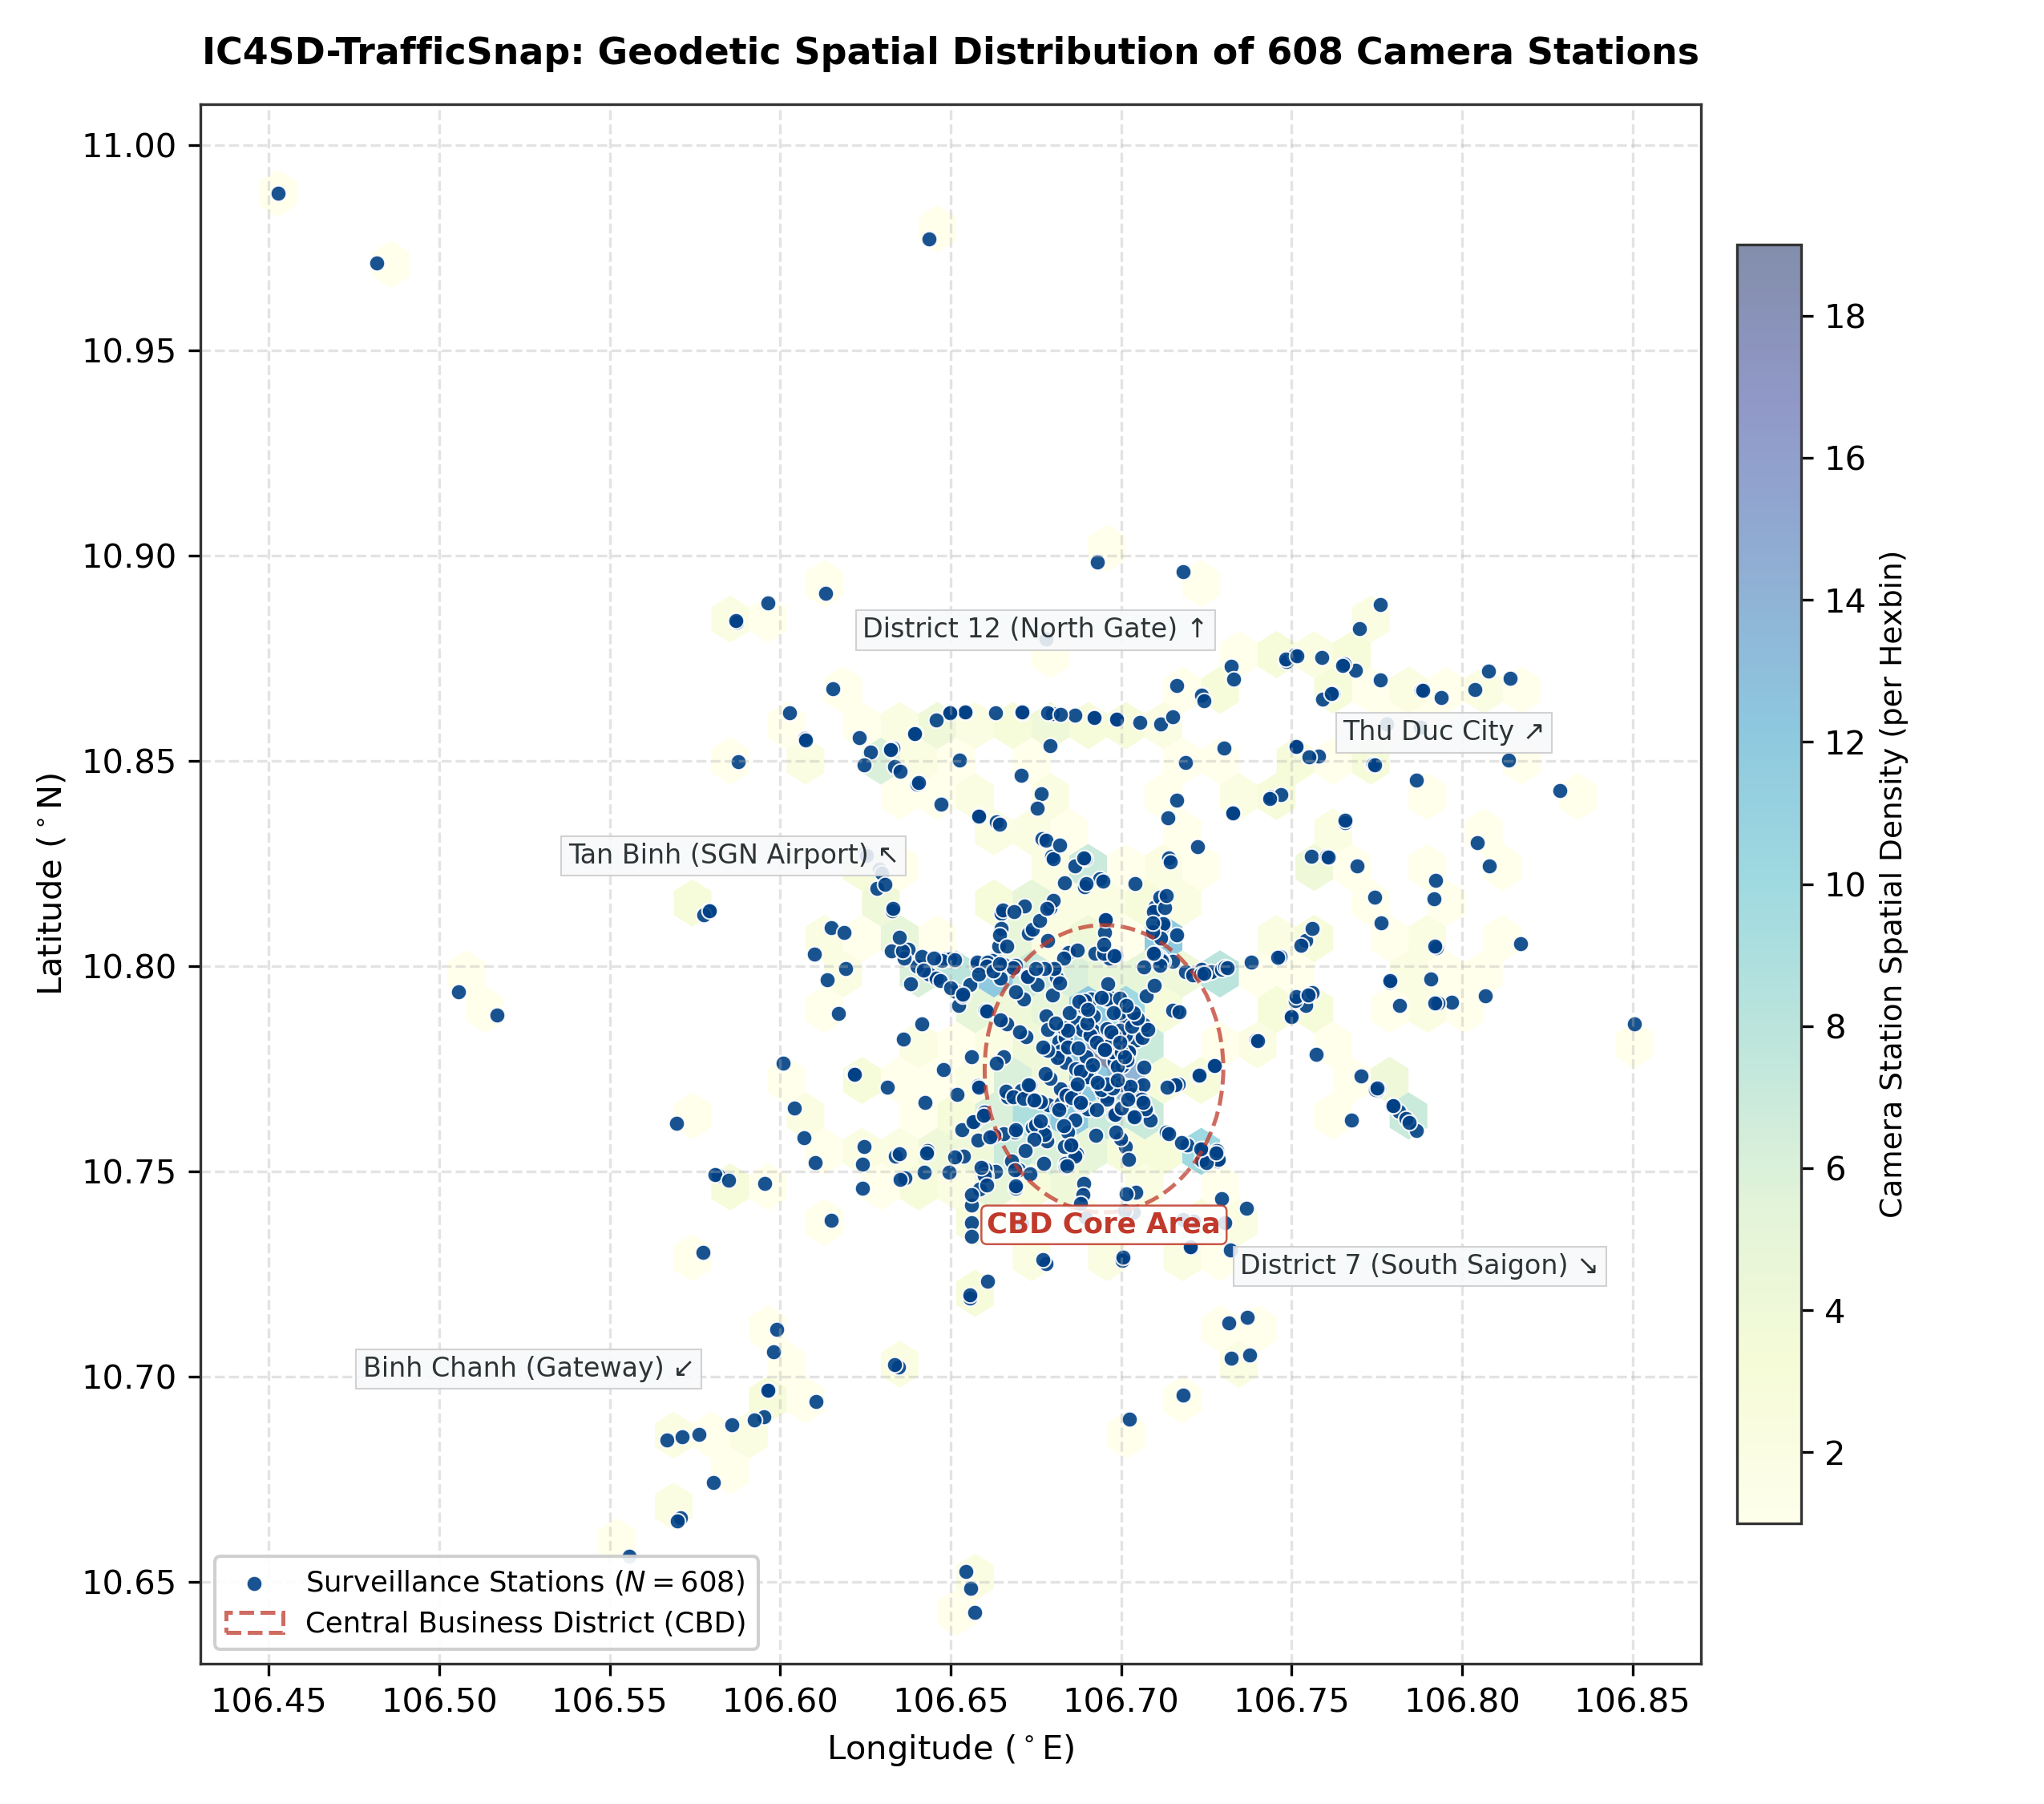
\includegraphics[width=0.88\textwidth]{direction_data_article/paper/figures/fig1_camera_spatial_map.png}
    \caption{\textbf{Bản đồ phân bố không gian của mạng lưới 608 trạm camera giám sát giao thông tại TP.HCM.} Hệ thống trạm quan sát bao phủ toàn diện các quận nội đô và vành đai đô thị, tập trung với mật độ cao tại các trục xuyên tâm, vòng xoay trọng điểm khu vực trung tâm và trải rộng dọc theo các tuyến cửa ngõ giao thương liên vùng.}
    \label{fig:camera_spatial_map}
\end{figure}

\begin{figure}[t!]
    \centering
    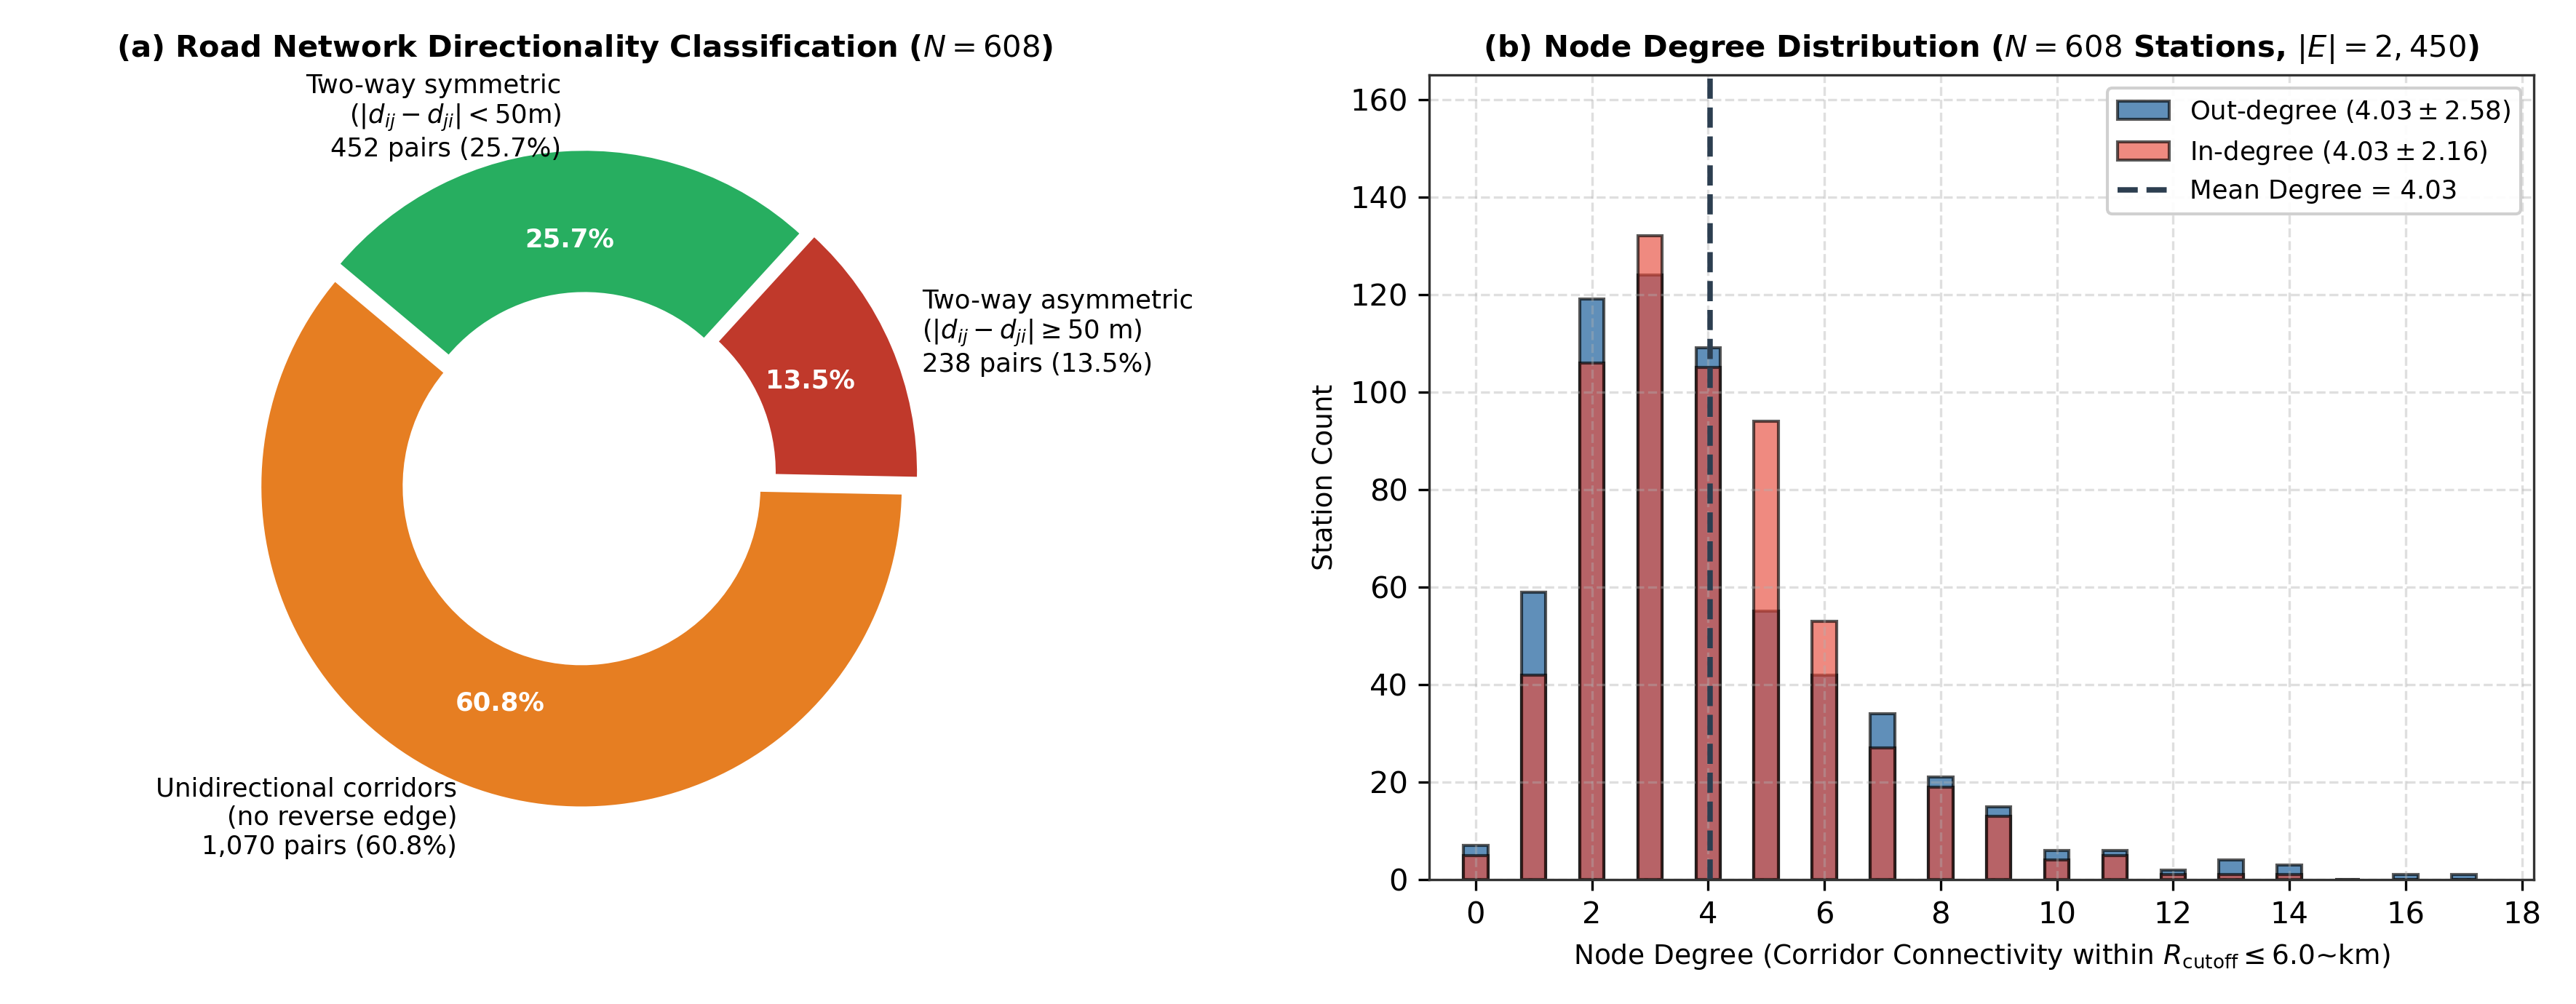
\includegraphics[width=0.95\textwidth]{direction_data_article/paper/figures/fig3_graph_topology.png}
    \caption{\textbf{Đặc trưng tô-pô đồ thị mạng lưới đường bộ OSRM trên mạng lưới 608 camera.} Phân tích 2,450 liên kết có hướng: (a) Phân bố cự ly di chuyển thực tế theo mạng đường giao thông; (b) Phân bố hệ số uốn khúc mạng lưới $\tau$ so với khoảng cách chim bay Haversine (trung bình $\tau = 1.25$); và (c) Phân bố độ lệch khoảng cách hai chiều $|d_{ij} - d_{ji}|$, làm nổi bật 238 cặp liên kết bất đối xứng cự ly $(\ge 50\text{ m})$ do mạng lưới sông ngòi chia cắt và hệ thống dải phân cách quay đầu xe đặc thù tại TP.HCM.}
    \label{fig:graph_topology}
\end{figure}

\begin{figure}[t!]
    \centering
    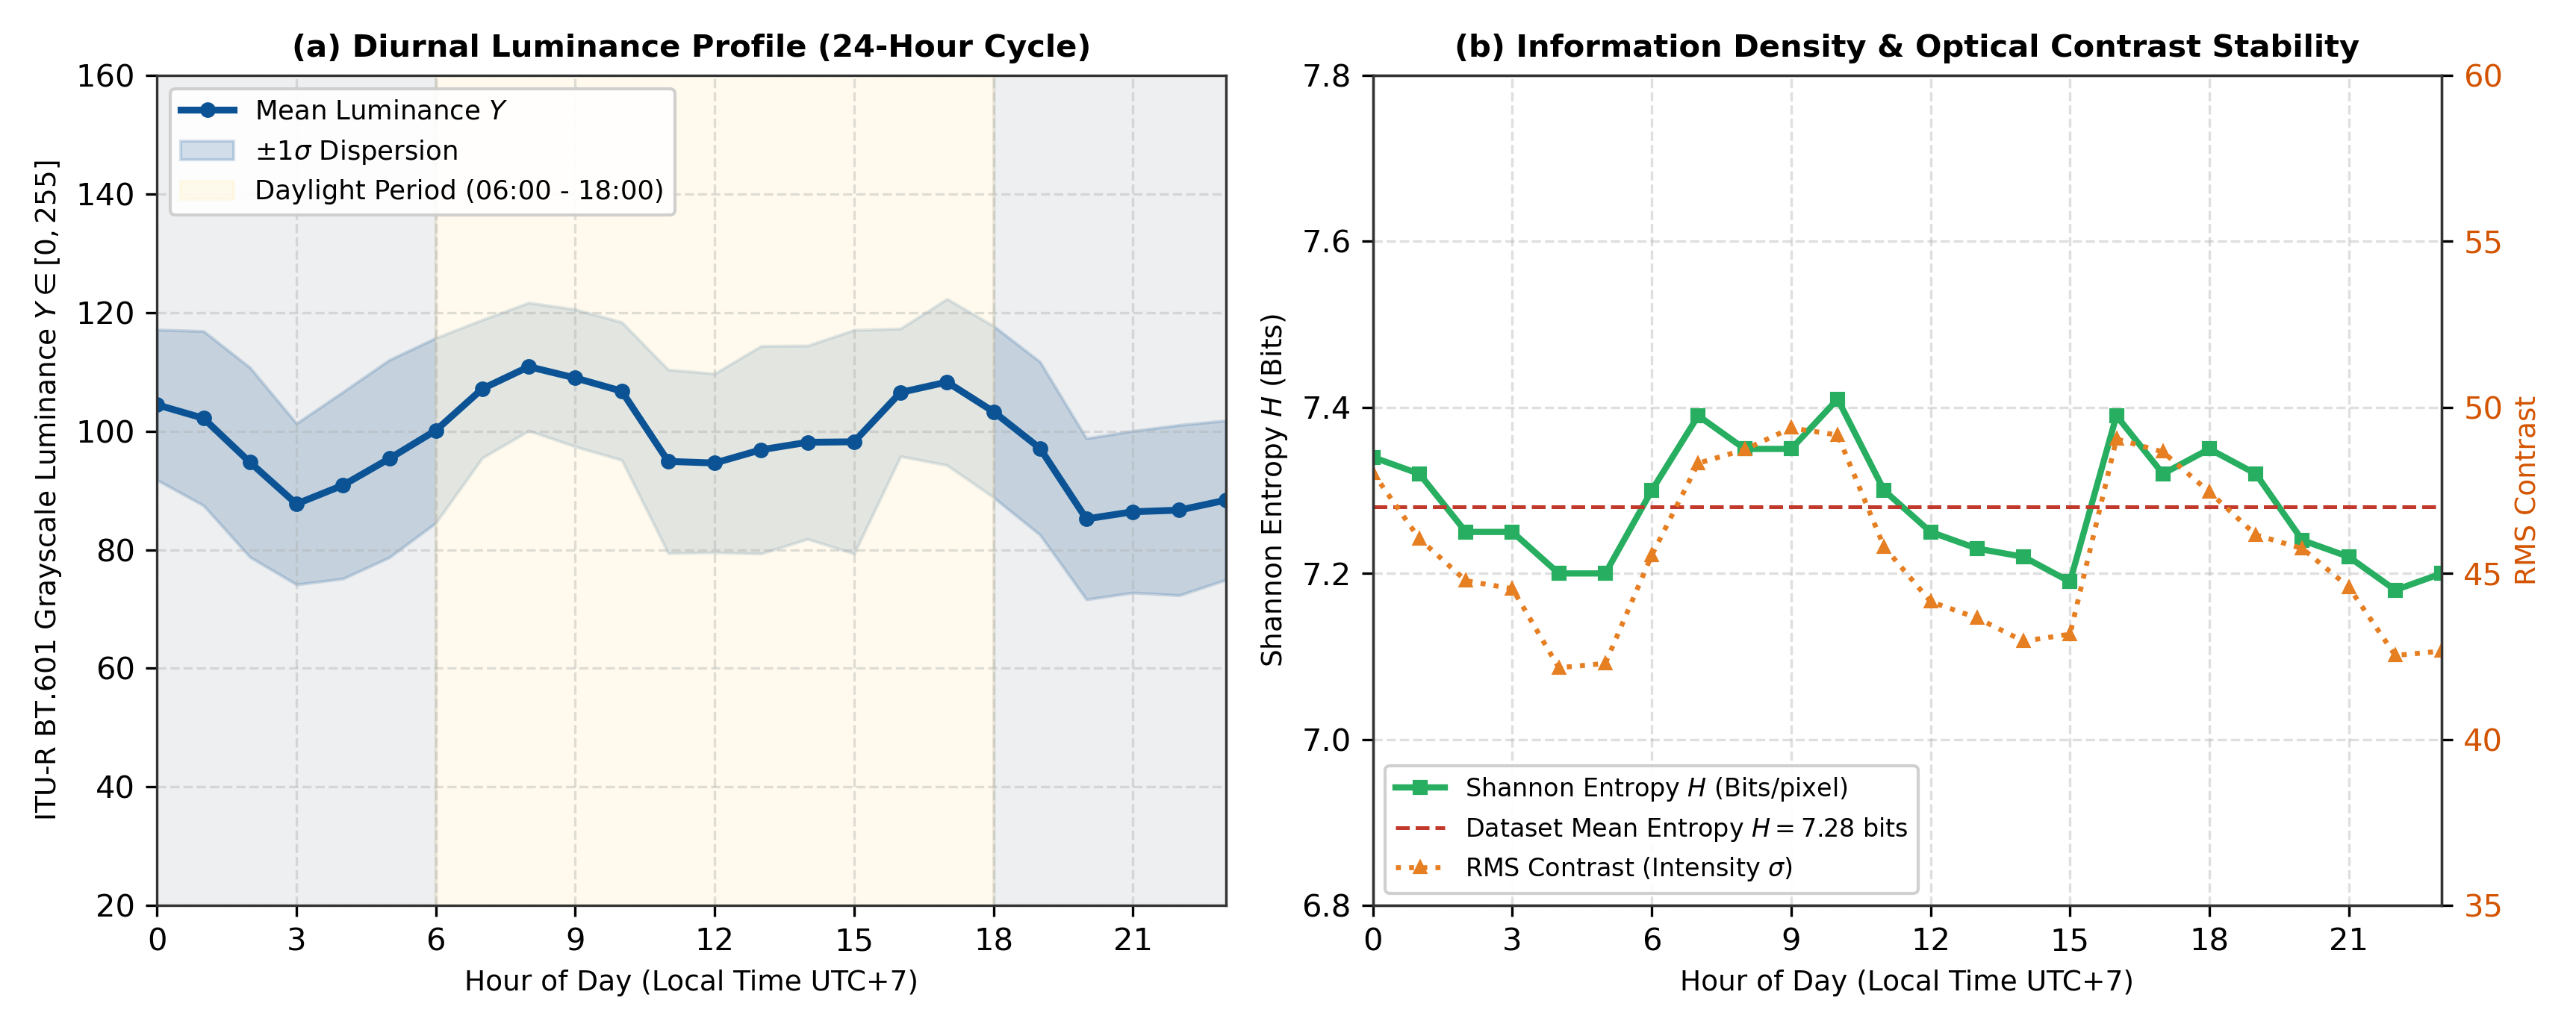
\includegraphics[width=0.95\textwidth]{direction_data_article/paper/figures/fig2_temporal_and_photometric.png}
    \caption{\textbf{Phân bố chu kỳ lấy mẫu thời gian và biến thiên trắc quang quang học.} (a) Phân bố chu kỳ làm mới khung hình $\Delta t$ phản ánh tính ngắt quãng đặc trưng với trung vị 240--270 giây và phân bố đuôi dài do giới hạn đường truyền diện rộng; (b) Phân bố độ sáng trung bình của ảnh hiện trường theo từng khung giờ trong ngày, thể hiện sự tương phản quang học sâu sắc giữa điều kiện ban ngày nhiệt đới và ban đêm đô thị.}
    \label{fig:temporal_photometric}
\end{figure}

\subsection{Kiểm Toán An Toàn Bảo Mật PII Theo Chuẩn Mực Sub-Nyquist}
Do dữ liệu thu thập từ các tuyến phố công cộng, việc bảo vệ quyền riêng tư cá nhân (Personally Identifiable Information -- PII) là một yêu cầu pháp lý và đạo đức khoa học bắt buộc. Tập dữ liệu IC4SD-TrafficSnap được thiết kế theo nguyên lý Bảo Mật Vật Lý Tự Thân (Physical Privacy by Design):
\begin{enumerate}
    \item \textbf{Giới hạn quang học Sub-Nyquist:} Với độ cao lắp đặt camera 6--15 m và cự ly quan sát 15--60 m, khoảng cách lấy mẫu mặt đất (Ground Sample Distance -- GSD) đạt mức $\text{GSD} \ge 2.73\text{ cm/pixel}$. Nét chữ trên biển số xe máy có bề rộng thực tế khoảng 0.5--1.0 cm, tương đương dưới $2\text{ pixel}$ trên ảnh cảm biến. Giới hạn này thấp hơn rất nhiều so với ngưỡng định lý lấy mẫu Nyquist cần thiết để nhận dạng ký tự quang học (OCR đòi hỏi tối thiểu $\ge 16\text{ pixel}$ cho mỗi ký tự).
    \item \textbf{Đặc thù văn hóa lưu thông:} Trên 85\% người điều khiển xe hai bánh tại TP.HCM sử dụng mũ bảo hiểm che kín trán và khẩu trang chống bụi, triệt tiêu hoàn toàn khả năng trích xuất đặc trưng sinh trắc học khuôn mặt.
    \item \textbf{Kiểm toán thống kê Rule of Three:} Quy trình kiểm toán ngẫu nhiên 200,000 khung hình độc lập và kiểm toán toàn bộ 714,123 khung hình ghi nhận 0 trường hợp vi phạm nhận dạng PII. Theo Quy tắc Thống kê Ba (Rule of Three), chặn trên khoảng tin cậy 95\% đối với tỷ lệ rủi ro nhận dạng PII trên toàn bộ tập dữ liệu là:
    \begin{equation}
        p_{95\%} \le \frac{3}{N} = \frac{3}{714,123} \approx 4.2 \times 10^{-6} \; (0.00042\%)
    \end{equation}
    bảo đảm tính an toàn pháp lý tuyệt đối để công bố dữ liệu mở cho cộng đồng nghiên cứu quốc tế.
\end{enumerate}

\section{KẾT LUẬN}
Hệ sinh thái DINO Traffic Suite đã thiết lập một hệ thống phương pháp luận hoàn chỉnh và chặt chẽ, phản ánh đầy đủ bức tranh tiến hóa từ các giải pháp khai thác tiền nghiệm nền trung vị truyền thống (Hướng 1 Cũ và Hướng 2 Cũ) đến các mũi nhọn tự học biểu diễn độc lập không cần nền (Hướng 1 Mới và Hướng 2 Mới), kết hợp cùng các mô hình suy luận phân tầng thích ứng ngữ cảnh đô thị (Hướng 3 và Hướng 4). Toàn bộ các công trình giải tích toán học, thuật toán lặp và cơ chế điều hòa đều bắt nguồn trực tiếp từ bản chất vật lý của dòng giao thông đô thị TP.HCM, đặt nền móng lý thuyết và thực nghiệm vững chắc cho các công bố khoa học quốc tế uy tín.

\end{document}
